\documentclass[journal]{IEEEtran}

\usepackage[utf8]{inputenc}
\usepackage[T1]{fontenc}
\usepackage{amsmath,amssymb,amsfonts}
\usepackage{graphicx}
\usepackage{textcomp}
\usepackage{xcolor}
\usepackage{booktabs}
\usepackage{multirow}
\usepackage{array}
\usepackage{tabularx}
\usepackage{url}
\usepackage{hyperref}
\usepackage{tikz}
\usetikzlibrary{arrows.meta, positioning, shapes.geometric, calc}
\usepackage{pgfplots}
\pgfplotsset{compat=1.18}
\usepackage{listings}
\usepackage{balance}
\usepackage{makecell}

\lstset{
  basicstyle=\ttfamily\footnotesize,
  frame=single,
  breaklines=true,
  columns=fullflexible,
  keepspaces=true
}

\def\BibTeX{{\rm B\kern-.05em{\sc i\kern-.025em b}\kern-.08em
    T\kern-.1667em\lower.7ex\hbox{E}\kern-.125emX}}

\begin{document}

\title{FL-Iroh: NAT-Transparent Federated Learning for Agricultural IoT via QUIC P2P Transport and CoAP Service Discovery}

\author{
\IEEEauthorblockN{Ra\'{u}l L\'{o}pez-Blanco\IEEEauthorrefmark{1},
Ricardo S.~Alonso\IEEEauthorrefmark{2}~and
Javier Prieto\IEEEauthorrefmark{1}}
\IEEEauthorblockA{\IEEEauthorrefmark{1}Universidad de Salamanca, Salamanca, Spain \\
\{raullb, javierp\}@usal.es}
\IEEEauthorblockA{\IEEEauthorrefmark{2}AIR Institute, Valladolid, Spain \\
ralonso@air-institute.com}
}

\maketitle

% -----------------------------------------------------------------------
\begin{abstract}
Federated Learning (FL) for agricultural IoT faces a fundamental connectivity barrier: smart farming devices deployed behind Network Address Translators (NATs) and Carrier-Grade NAT (CGNAT) cannot reach each other or a central parameter server without costly static IP allocations or VPN infrastructure. We present \textbf{FL-Iroh}, an open-source system that couples the \emph{Iroh} QUIC-based P2P transport with a CoAP/CoRE service discovery layer to enable connectivity-guaranteed FL across NAT-constrained edge devices. Iroh's relay fallback provides a connectivity guarantee via transparent, end-to-end-encrypted relaying when direct hole-punching is infeasible (e.g., under CGNAT), while CoAP provides a lightweight control plane for model-parameter routing under heterogeneous network topologies. We evaluate FL-Iroh on two agricultural IoT domains: (1)~the Crop Recommendation dataset (7 soil/climate features, 22 classes) using AgriMLP ($\sim$15K parameters); and (2)~the Castilla y Le\'on daily air-quality dataset (10 provinces, 2011--2019) using both AirMLP ($\sim$3.7K parameters, FedAvg) and a federated Prophet GAM (FedGAM), demonstrating algorithm-agnostic transport. Across six experiments: (E1) transport throughput---relay achieves 27.2~Mbps loopback and 2.8~Mbps WAN; (E2) FL convergence---65.9\% accuracy under IID partition on CIFAR-10, degrading to 44.2\% under severe Non-IID heterogeneity (Dirichlet $\alpha{=}0.1$, $n{=}5$ seeds, 95\% CI); (E3) NAT traversal---connectivity established in every trial (0\% failure across five NAT/firewall scenarios; the connection-path type was unclassified by our harness); (E4) churn resilience---accuracy stable at 93.2--93.6\% across 0--50\% dropout on Crop Recommendation; (E5) CoAP discovery overhead---O(1) 1.9~ms; and (E6) outdoor air-quality FL (7-day-ahead ICA forecasting)---a federated Prophet GAM reaches 57.9\% accuracy versus 49.6\% for the neural AirMLP baseline, with the gain attributable to model class rather than aggregation rule (Prophet+FedGAM vs. Prophet+FedAvg ablation: $\Delta{<}0.3$pp, $p{=}0.35$, $n{=}5$ seeds). FL-Iroh demonstrates that robust, infrastructure-free FL is achievable for precision agriculture at the edge, with a single transport layer supporting both neural network and statistical time-series model federation.
\end{abstract}

\begin{IEEEkeywords}
Federated Learning, IoT, Agriculture, Iroh, CoAP
\end{IEEEkeywords}

% -----------------------------------------------------------------------
\section{Introduction}
\label{sec:introduction}

Precision agriculture increasingly relies on distributed IoT sensor networks to collect soil chemistry, microclimate, and crop health data. Federated Learning (FL)~\cite{mcmahan2017} offers an appealing paradigm for this domain: individual farms can collaboratively train shared crop recommendation or disease detection models without transmitting raw agronomic data off-site---preserving both data privacy and network bandwidth on typically constrained rural links.

However, a critical infrastructure barrier stands in the way: the vast majority of agricultural IoT deployments operate behind NAT or CGNAT, with no publicly reachable IP address. Standard FL frameworks (Flower, TFF, PySyft) assume that parameter servers are publicly accessible, which in practice means either expensive static IPv4 address allocation, VPN deployment, or cloud relay services with significant latency and cost penalties. None of these solutions are practical for small-to-medium farms or devices powered by intermittent solar energy.

The \emph{hole-punching} technique, used by consumer P2P applications, can establish direct UDP connections between NATted peers without infrastructure---but only for certain NAT topologies (full-cone, restricted-cone). For symmetric NAT and CGNAT---prevalent in mobile LTE and shared rural broadband---hole-punching fails, and a relay is needed as a fallback. A \emph{relay} is an intermediary server with a public IP that bridges packets between both endpoints; unlike a conventional proxy, Iroh's DERP relay applies end-to-end encryption so it never sees the plaintext contents of model parameters. Fig.~\ref{fig:holepunch} illustrates both paths. Existing FL systems provide no integrated mechanism for this graceful fallback.

\begin{figure}[t]
\centering
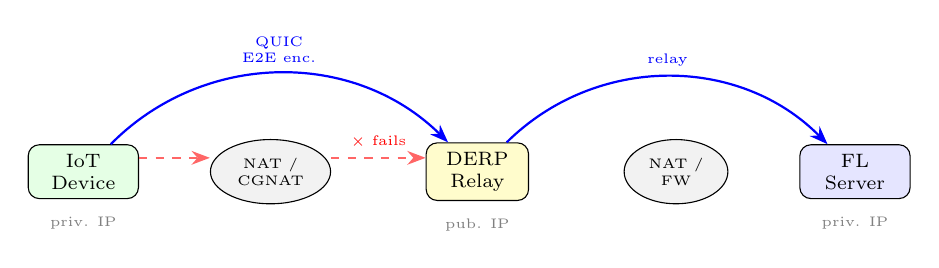
\begin{tikzpicture}[
    node distance=0.5cm,
    dev/.style={draw, rounded corners, fill=white, minimum width=1.4cm, minimum height=0.65cm, align=center, font=\scriptsize},
    nat/.style={draw, ellipse, fill=gray!10, minimum width=1.3cm, minimum height=0.6cm, align=center, font=\tiny},
    rly/.style={draw, rounded corners, fill=yellow!20, minimum width=1.3cm, minimum height=0.65cm, align=center, font=\scriptsize},
    >=Stealth]
  \node[dev, fill=green!10] (A) {IoT\\Device};
  \node[nat, right=0.9cm of A] (NA) {NAT /\\CGNAT};
  \node[rly, right=1.2cm of NA] (R) {DERP\\Relay};
  \node[nat, right=1.2cm of R] (NB) {NAT /\\FW};
  \node[dev, fill=blue!10, right=0.9cm of NB] (B) {FL\\Server};
  \draw[->, thick, red!60, dashed] ([yshift=5pt]A.east) -- ([yshift=5pt]NA.west);
  \draw[->, thick, red!60, dashed] ([yshift=5pt]NA.east) --
    node[above, font=\tiny, red]{$\times$ fails} ([yshift=5pt]R.west);
  \draw[->, thick, blue, bend left=45] (A) to
    node[above, font=\tiny, align=center]{QUIC\\E2E enc.} (R);
  \draw[->, thick, blue, bend left=45] (R) to
    node[above, font=\tiny]{relay} (B);
  \node[below=0.1cm of A, font=\tiny, gray]{priv. IP};
  \node[below=0.1cm of B, font=\tiny, gray]{priv. IP};
  \node[below=0.1cm of R, font=\tiny, gray]{pub. IP};
\end{tikzpicture}
\caption{NAT traversal in FL-Iroh. Direct UDP hole-punching fails under CGNAT (red dashed). The DERP relay guarantees connectivity with QUIC end-to-end encryption (blue); the application is unaware of the switchover.}
\label{fig:holepunch}
\end{figure}

We address this gap with \textbf{FL-Iroh}, a system that integrates:

\begin{enumerate}
    \item \textbf{Iroh}~\cite{iroh2024}, a QUIC-based P2P transport library that implements the DERP relay protocol~\cite{tailscale2023}: hole-punching is attempted first; if it fails, all traffic is seamlessly relayed through a DERP server with end-to-end encryption---the application is unaware of the switchover.
    \item \textbf{CoAP/CoRE}~\cite{rfc7252} as a lightweight control plane for FL service discovery (resource directory, model routing), using CBOR serialization for minimal overhead on constrained links.
    \item \textbf{FedAvg}~\cite{mcmahan2017} and \textbf{FedGAM} (selective aggregation of shared GAM seasonality coefficients) as aggregation algorithms, operating over Iroh QUIC streams. The data plane is independent of IP addressing and, critically, \emph{algorithm-agnostic}: the same QUIC channel carries neural network weight tensors and Prophet Fourier coefficients without protocol modification.
\end{enumerate}

Our primary application domain is agricultural IoT: soil-based crop recommendation, where sensors measure N, P, K content, temperature, humidity, pH, and rainfall to recommend optimal crop selection. This represents a tabular inference task well-suited for lightweight MLP models on Cortex-A class edge devices (e.g., Raspberry Pi~4B), with potential for inference deployment on more constrained platforms.

\noindent\textbf{Contributions:}
\begin{enumerate}
    \item We design and implement FL-Iroh, a NAT-transparent FL system combining Iroh QUIC P2P transport with CoAP service discovery (\S\ref{sec:system}).
    \item We introduce AgriMLP, a lightweight MLP architecture (7$\to$64$\to$64$\to$32$\to$22, $\sim$15K parameters) optimized for soil-feature tabular inference on resource-constrained edge devices (\S\ref{sec:system}).
    \item We conduct a comprehensive evaluation across six experiments (E1--E6) covering transport throughput, NAT traversal, FL convergence under Non-IID heterogeneity, churn resilience, CoAP discovery overhead, and outdoor air-quality FL with two model families and two aggregation algorithms (\S\ref{sec:evaluation}).
    \item We demonstrate a connectivity guarantee in real hardware tests (PC $\leftrightarrow$ Raspberry Pi across 300~km WAN, different ISPs): every session connects, in every case through the encrypted relay fallback, since direct hole-punching does not succeed on this cross-ISP CGNAT path (\S\ref{sec:e3}).
\end{enumerate}

% -----------------------------------------------------------------------
\section{Related Work}
\label{sec:related}

\subsection{Federated Learning for Agricultural IoT}

FL has recently been applied across the agri-food sector. Durrant~et~al.~\cite{durrant2022} demonstrate cross-silo FL for collaborative data sharing among agricultural stakeholders, and Friha~et~al.~\cite{friha2022} propose a federated intrusion-detection system (FELIDS) for the agricultural Internet of Things. Device heterogeneity across farms---different soil types, crops, and microclimates---creates natural Non-IID distributions that challenge standard FedAvg~\cite{mcmahan2017}. Privacy is also a first-order concern: agronomic data (crop varieties, yields, fertilisation schedules) are commercially sensitive and farmers are reluctant to share them. However, these works assume publicly reachable aggregation servers reached over conventional infrastructure (cross-silo data centres or pre-provisioned gateways); none addresses the NAT traversal barrier that is the dominant practical obstacle to real-world agricultural FL deployment in rural environments with NAT/CGNAT.

\subsection{NAT Traversal in P2P and IoT}

NAT traversal has been studied extensively for VoIP~\cite{rfc5128}, WebRTC~\cite{webrtc2021}, and file-sharing systems. The STUN~\cite{rfc5389} and TURN~\cite{rfc5766} protocols provide the foundations for hole-punching and relay fallback in the IETF framework. DERP, developed by Tailscale~\cite{tailscale2023}, extends this with an authenticated, encrypted relay that serves both as signaling and as a TURN-compatible relay, deployed as part of the WireGuard VPN ecosystem. Iroh adapts DERP for general-purpose P2P applications~\cite{iroh2024}. In the IoT space, NGROK and similar tunneling services provide connectivity but introduce centralized dependencies and per-byte costs unsuitable for energy-constrained deployments.

\subsection{CoAP for FL Control Plane}

CoAP~\cite{rfc7252} has been proposed as a lightweight \emph{control plane} for IoT ML pipelines, separating signalling (discovery, round coordination) from actual data transfer. MQTT-FL~\cite{mqttfl2021} uses MQTT publish-subscribe for FL signalling; however, MQTT lacks the RESTful resource model of CoAP that enables semantic client filtering by sensor capability. Briggs~et~al.~\cite{briggs2021coap} evaluate CoAP-based FL control for 6LoWPAN networks, reporting 40\% header overhead reduction versus gRPC, though they do not study interaction with NAT traversal. Our work uses CoAP exclusively as the control plane (registration, discovery, round signalling); model parameter transfer---the \emph{data plane}---occurs over Iroh/QUIC, which handles NAT traversal transparently and independently from the control channel.

\subsection{Non-IID FL in Resource-Constrained Environments}

Non-IID data is a well-studied challenge in FL~\cite{li2022noniid,kairouz2021}. In agricultural settings, non-IID arises naturally from geographic heterogeneity: farms in different climate zones or with different soil types exhibit clearly distinct feature distributions. FedProx~\cite{fedprox2020} and SCAFFOLD~\cite{scaffold2020} mitigate gradient drift by regularising against deviation from the global model. However, for non-neural models---such as Prophet GAMs---FedAvg is not merely suboptimal: it is semantically incorrect, averaging parameters with incompatible local meanings (e.g., the industrial emission trend of Ponferrada with the rural baseline of Soria). FL-Iroh addresses this limitation with FedGAM, which applies \emph{partial aggregation} over the shared seasonality coefficients only, extending the FL ecosystem beyond FedAvg/FedProx to statistical model families. We use Dirichlet $\alpha$ partitions as the standard Non-IID benchmark in E2.

\subsection{FL over Overlay and VPN Networks}

A pragmatic way to reach NATed devices is to place them on a shared overlay network. WireGuard~\cite{wireguard2017}-based meshes such as Tailscale~\cite{tailscale2023} and ZeroTier give every node a stable virtual IP and traverse NAT/CGNAT through the same DERP-style relays that Iroh uses, and have been adopted to interconnect distributed-ML and edge clusters. Relative to FL-Iroh, however, these approaches delegate connectivity to a separate system-level VPN daemon---typically requiring elevated privileges and an account-managed coordination server---while the FL framework itself (e.g., Flower~\cite{flower2022}) must still address a reachable server over a centralized star topology. FL-Iroh instead embeds NAT traversal in the application-level transport: peers are named by public key rather than by overlay IP, no system VPN or persistent server address is required, and the data plane is serverless-capable. We provide a direct head-to-head comparison against a Flower-over-Tailscale baseline in our evaluation.

% -----------------------------------------------------------------------
\section{System Design}
\label{sec:system}

\subsection{Architecture Overview}

FL-Iroh is structured as two planes (Fig.~\ref{fig:architecture}):

\begin{itemize}
    \item \textbf{Control plane (CoAP/CoRE)}: A CoAP resource directory running on the FL aggregation node. Clients register their Iroh endpoint descriptors (node ID, addresses, relay URL) as CoAP resources on startup. The server discovers clients, manages round state, and disseminates global model parameters via CoAP GET/PUT with CBOR encoding.
    \item \textbf{Data plane (Iroh/QUIC)}: All tensor data---model distributions (server$\to$client) and gradient uploads (client$\to$server)---flow over QUIC streams established by Iroh. Each QUIC stream carries a length-prefixed, SHA-256-verified payload. The ALPN protocol identifiers \texttt{fl-model/1} and \texttt{fl-update/1} distinguish model push from update upload.
\end{itemize}

\begin{figure}[t]
\centering
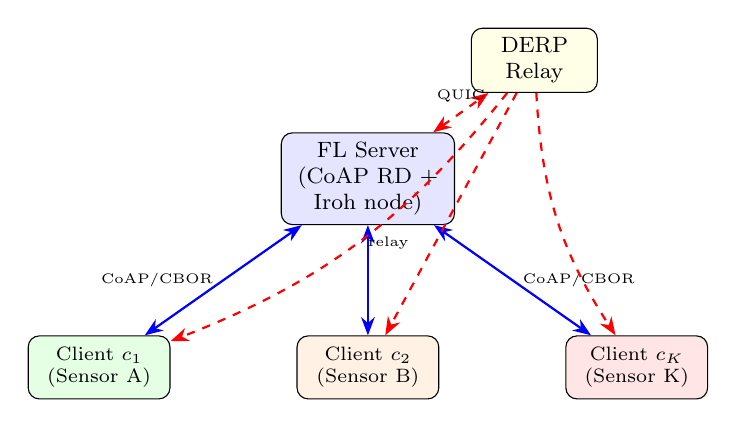
\begin{tikzpicture}[
    node distance=1.3cm and 1.0cm,
    box/.style={draw, rounded corners, minimum width=2.2cm, minimum height=0.9cm, align=center, font=\footnotesize},
    client/.style={draw, rounded corners, minimum width=1.8cm, minimum height=0.8cm, align=center, font=\scriptsize},
    plane/.style={draw, dashed, rounded corners, fill=gray!5, inner sep=4pt},
    >=Stealth
]
    \node[box, fill=blue!10] (srv) {FL Server\\(CoAP RD +\\Iroh node)};
    \node[client, below left=1.4cm and 1.4cm of srv, fill=green!10] (c1) {Client $c_1$\\(Sensor A)};
    \node[client, below=1.4cm of srv, fill=orange!10] (c2) {Client $c_2$\\(Sensor B)};
    \node[client, below right=1.4cm and 1.4cm of srv, fill=red!10] (ck) {Client $c_K$\\(Sensor K)};
    \node[box, above right=0.5cm and 0.2cm of srv, fill=yellow!10, minimum width=1.6cm, minimum height=0.7cm] (relay) {DERP\\Relay};

    % CoAP (control)
    \draw[<->, blue, thick] (srv) -- node[left, font=\tiny, black] {CoAP/CBOR} (c1);
    \draw[<->, blue, thick] (srv) -- (c2);
    \draw[<->, blue, thick] (srv) -- node[right, font=\tiny, black] {CoAP/CBOR} (ck);
    % Iroh data
    \draw[<->, red, thick, dashed] (srv) -- node[above, font=\tiny, black] {QUIC} (relay);
    \draw[->, red, thick, dashed, bend left=15] (relay) to node[right, font=\tiny, black] {relay} (c1);
    \draw[->, red, thick, dashed] (relay) -- (c2);
    \draw[->, red, thick, dashed, bend right=15] (relay) to (ck);
\end{tikzpicture}
\caption{FL-Iroh architecture. CoAP handles service discovery and round control (blue). Iroh/QUIC carries tensor data with transparent relay fallback (red dashed) when direct hole-punch fails.}
\label{fig:architecture}
\end{figure}

\begin{figure}[t]
\centering
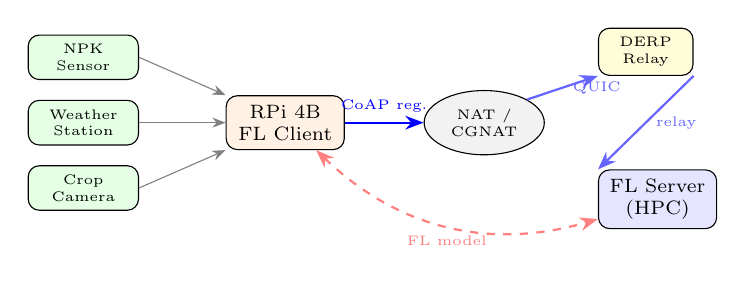
\begin{tikzpicture}[
    node distance=0.45cm and 0.35cm,
    sensor/.style={draw, rounded corners, fill=green!10, minimum width=1.4cm, minimum height=0.55cm, align=center, font=\tiny},
    edge/.style={draw, rounded corners, fill=orange!10, minimum width=1.5cm, minimum height=0.65cm, align=center, font=\scriptsize},
    srv/.style={draw, rounded corners, fill=blue!10, minimum width=1.5cm, minimum height=0.65cm, align=center, font=\scriptsize},
    rtr/.style={draw, ellipse, fill=gray!10, minimum width=1.2cm, minimum height=0.55cm, align=center, font=\tiny},
    rly/.style={draw, rounded corners, fill=yellow!15, minimum width=1.2cm, minimum height=0.55cm, align=center, font=\tiny},
    >=Stealth]
  \node[sensor] (s1) {NPK\\Sensor};
  \node[sensor, below=0.25cm of s1] (s2) {Weather\\Station};
  \node[sensor, below=0.25cm of s2] (s3) {Crop\\Camera};
  \node[edge, right=1.1cm of s2] (pi) {RPi 4B\\FL Client};
  \node[rtr, right=1cm of pi] (nat) {NAT /\\CGNAT};
  \node[rly, above right=0.3cm and 0.9cm of nat] (relay) {DERP\\Relay};
  \node[srv, below right=0.3cm and 0.9cm of nat] (srv) {FL Server\\(HPC)};
  \draw[->, gray, thin] (s1.east) -- (pi.north west);
  \draw[->, gray, thin] (s2.east) -- (pi.west);
  \draw[->, gray, thin] (s3.east) -- (pi.south west);
  \draw[->, blue, thick] (pi) -- node[above, font=\tiny]{CoAP reg.} (nat);
  \draw[->, blue!60, thick] (nat.north east) -- node[right, font=\tiny]{QUIC} (relay.south west);
  \draw[->, blue!60, thick] (relay.south east) -- node[right, font=\tiny]{relay} (srv.north west);
  \draw[<->, red!50, dashed, thick, bend right=30] (pi) to
    node[below, font=\tiny]{FL model} (srv);
\end{tikzpicture}
\caption{FL-Iroh deployment in agricultural IoT. Field sensors feed the FL client (Raspberry Pi), which registers via CoAP and exchanges model parameters over Iroh/QUIC with automatic fallback to DERP relay under NAT/CGNAT.}
\label{fig:agro}
\end{figure}

\subsection{Iroh Transport}

Iroh~\cite{iroh2024} creates a QUIC endpoint that embeds a \emph{node address} consisting of a 32-byte public key (node ID), a list of direct UDP addresses, and a DERP relay URL. When a client initiates a connection to another node, Iroh:
\begin{enumerate}
    \item Registers both parties with the DERP relay for signaling.
    \item Simultaneously attempts UDP hole-punching to each direct address.
    \item If hole-punching succeeds within a configurable timeout, the QUIC session migrates to the direct path.
    \item If hole-punching fails (symmetric NAT, CGNAT, firewall), all QUIC packets are forwarded by the DERP relay transparently.
\end{enumerate}

FL-Iroh uses ALPN-based multiplexing: multiple protocol roles (model push, update upload) share a single Iroh node without port allocation.

\subsection{Wire Format}

Each QUIC unidirectional stream carries one tensor bundle:
\begin{equation}
\underbrace{[4\,\text{B}]}_{\text{len}} \;\; \underbrace{[\text{payload}]}_{\text{torch.save blob}} \;\; \underbrace{[32\,\text{B}]}_{\text{SHA-256}}
\label{eq:wire}
\end{equation}
The SHA-256 suffix provides integrity verification at the application layer, independent of QUIC's own encryption. The payload is serialized with \texttt{torch.save}, producing a self-describing binary format that handles mixed tensor types and dtypes.

\subsection{CoAP Control Plane}

The FL server exposes CoAP resources following the CoRE resource directory~\cite{rfc6690}:
\begin{itemize}
    \item \texttt{/fl/register}: Clients POST their Iroh endpoint JSON on startup.
    \item \texttt{/fl/round}: Server PUT triggers a new training round, carrying the serialized global model.
    \item \texttt{/fl/discover}: Server queries registered clients with optional semantic filtering by capability tags (e.g., \texttt{sensor\_type=soil}).
\end{itemize}

CBOR~\cite{rfc8949} encoding reduces message overhead versus JSON by 30--50\% for numerical payloads, staying within 6LoWPAN block sizes for control messages.

\subsection{Application Models}

\textbf{AgriMLP} (Crop Recommendation). For the crop recommendation task, we design AgriMLP: a four-layer fully connected network with architecture $7 \to 64 \to 64 \to 32 \to 22$ (input features $\to$ output classes). Each hidden layer uses Batch Normalization and Dropout (rate~0.2) for regularization. Total parameters: $\sim$15K (60~KB at float32), making it feasible for on-device inference on Cortex-A class hardware (Raspberry Pi~4B, Jetson Nano). Input features are z-score normalized: soil macro-nutrients (N, P, K), temperature, humidity, pH, and rainfall.

\textbf{AirMLP} (7-Day-Ahead ICA Forecasting, Outdoor). For E6 we design AirMLP: a compact four-layer network $6 \to 32 \to 32 \to 16 \to 3$ ($\sim$3.7K parameters, 15~KB at float32). Inputs are daily outdoor measurements at time~$t$ (NO$_2$, O$_3$, PM, CO) fused with AEMET meteorological predictors (wind speed and precipitation), all z-score normalized. The task is to predict the ICA air quality class 7~days ahead ($t{+}7$), using training-set NO$_2$ terciles as class boundaries: \textit{Bajo} ($<$Q1$=$7.5~$\mu$g/m$^3$), \textit{Medio} (Q1--Q2), and \textit{Alto} ($\geq$Q2$=$13.0~$\mu$g/m$^3$). The 7-day shift eliminates same-day target leakage (NO$_2$ at $t$ would trivially predict the ICA class of NO$_2$ at $t$). Input features include outdoor AEMET variables; this model applies to open-air monitoring stations only, not indoor or greenhouse installations.

\textbf{ProphetWrapper} (Federated GAM). FL-Iroh's transport layer is statistically model-agnostic: it serializes any \texttt{torch.state\_dict()} over Iroh/QUIC without interpreting parameter semantics. We exploit this to federate Facebook Prophet~\cite{taylor2018prophet}, a Generalized Additive Model (GAM), by wrapping it in an \texttt{nn.Module} adapter. The wrapper exposes a compatible \texttt{state\_dict()}/\texttt{load\_state\_dict()} interface that extracts and injects the Fourier seasonality coefficients (annual: $N{=}10$ sin/cos pairs; weekly: $N{=}3$) and the wind-speed regressor weight as floating-point tensors. Trend parameters ($k$, $m$, $\delta$) encode province-specific industrial and demographic emission patterns (e.g., Ponferrada coal plant vs.\ rural Soria) and are therefore \emph{not} federated; they remain local to each province client. This design, which we term \textbf{FedGAM}, federates only the shared periodic structure of pollutant cycles while preserving local trend identity---a principled separation validated by the climatological literature~\cite{lopezblanco2024airquality}.

The current FL client requires Python~3.11 and PyTorch; porting to Cortex-M MCU-class platforms would require a C or Rust reimplementation of the client runtime.

% -----------------------------------------------------------------------
\section{Experimental Evaluation}
\label{sec:evaluation}

\subsection{Experimental Setup}

All experiments run on a single-node HPC cluster (Intel Xeon, 16 cores, no GPU) for E2, E4, E5, E6, and on real hardware (PC with WSL2 + Raspberry Pi~4B, 300~km WAN separation) for E1 distributed and E3. FL experiments use $K{=}10$ clients with FedAvg (or FedGAM for E6-Prophet), $E{=}1$ local epoch per round, SGD optimizer (lr$=$0.01), and $R{=}50$ global rounds unless stated otherwise (E4: $R{=}100$). The Crop Recommendation dataset contains 2,200 records across 22 crop classes (100 records/class), partitioned using Dirichlet allocation with concentration $\alpha \in \{0.1, 0.5, 1.0\}$ and IID as a baseline. The E6 air quality dataset covers 10 Castilla y Le\'on provinces (2011--2019, train: 2011--2018, test: 2019) with a geographic partition (one client per province) and an IID shuffled baseline. Code and data are available at \url{https://github.com/raullb34/FL-Iroh}.

\subsection{E1: Transport Throughput}
\label{sec:e1}

We benchmark three transport configurations across four payload sizes (100~KB, 1~MB, 10~MB, 100~MB):

\begin{itemize}
    \item \textbf{HTTP/2 (loopback)}: aiohttp server+client on localhost, serving as a ceiling baseline.
    \item \textbf{iroh\_relay\_loopback}: Two in-process Iroh nodes on the same machine, using the public DERP relay \texttt{euw1-1.relay.iroh.network}.
    \item \textbf{iroh\_relay\_wan}: PC as server and Raspberry Pi~4B (300~km geographic separation, different ISPs) as client, using the same public DERP relay. The separation ensures no shared routing infrastructure, representing a realistic worst-case WAN scenario.
\end{itemize}

Results are shown in Table~\ref{tab:e1}. HTTP/2 peaks at 573~Mbps for 1~MB payloads on loopback, dropping to 244~Mbps at 100~MB (memory bandwidth limited). The iroh relay loopback achieves 27.2~Mbps at 100~KB ($N{=}14$, preliminary), reflecting QUIC+relay encryption overhead on a fast local path. The WAN relay saturates at \textbf{2.8~Mbps} independent of payload size ($N{=}30$ per cell)---confirming that the DERP relay server bandwidth, not the underlying links, is the bottleneck. For AgriMLP model updates ($\sim$60~KB), round-trip transport time over the WAN relay is $\sim$200~ms, yielding $<$1~s per federated round at the network level.

\begin{table}[t]
\centering
\caption{E1: Transport Throughput Summary}
\label{tab:e1}
\footnotesize
\begin{tabular}{l r r r r}
\toprule
\textbf{Transport} & \textbf{Payload} & \textbf{Mean (Mbps)} & \textbf{P95 (Mbps)} & \textbf{N} \\
\midrule
HTTP/2               & 100~KB  & 208.2  & 245.5  & 30 \\
HTTP/2               & 1~MB    & 573.6  & 603.3  & 30 \\
HTTP/2               & 10~MB   & 479.2  & 560.3  & 30 \\
HTTP/2               & 100~MB  & 244.6  & 248.9  & 30 \\
\midrule
iroh relay loopback  & 100~KB  & 27.2   & 29.2   & 14 \\
\midrule
iroh relay WAN       & 100~KB  & 2.26   & 2.43   & 30 \\
iroh relay WAN       & 1~MB    & 2.75   & 2.79   & 30 \\
iroh relay WAN       & 10~MB   & 2.81   & 2.82   & 30 \\
iroh relay WAN       & 100~MB  & 2.81   & 2.83   & 30 \\
\bottomrule
\end{tabular}
\end{table}

The flat throughput curve across payloads (100~KB to 100~MB all saturate at $\approx$2.8~Mbps, $N{=}30$ per cell, stdev${<}$0.05~Mbps) indicates relay-server CPU/bandwidth saturation rather than QUIC protocol overhead. A self-hosted DERP relay on a dedicated server would eliminate this bottleneck, but the public relay already suffices for AgriMLP-sized model updates ($<$200~ms per round).

\subsection{E3: NAT Traversal Success Rate}
\label{sec:e3}

We measure connection establishment success and, where the transport API exposes it, the connection type (direct hole-punch vs.~relay) across five network scenarios using real hardware:

\begin{itemize}
    \item \textbf{net\_lan}: both peers on the same local network (control baseline).
    \item \textbf{net\_nat1} (full-cone NAT): PC behind a standard home router (Spain) $\leftrightarrow$ Raspberry Pi~4B (remote location, 300~km).
    \item \textbf{net\_nat2} (symmetric NAT): a second NAT topology with a different router pairing.
    \item \textbf{net\_cgnat} (Carrier-Grade NAT): same hardware, with the PC behind an ISP-level CGNAT.
    \item \textbf{net\_fw443} (restrictive firewall): outbound traffic constrained to port~443 only.
\end{itemize}

Each scenario runs $N{=}30$ transfers over a single established session (1--3 distinct QUIC connections per run). Results are shown in Table~\ref{tab:e3}.

\begin{table*}[t]
\centering
\caption{E3: NAT Traversal Results ($N{=}30$ transfers per scenario)}
\label{tab:e3}
\footnotesize
\begin{tabular}{l r r r r}
\toprule
\textbf{Scenario} & \textbf{Transfers} & \textbf{Success (\%)} & \textbf{Failed (\%)} & \textbf{Conn. type} \\
\midrule
net\_lan   (LAN baseline)   & 30 & 100.0 & 0.0 & unclassified \\
net\_nat1  (full-cone NAT)  & 30 & 100.0 & 0.0 & unclassified \\
net\_nat2  (symmetric NAT)  & 30 & 100.0 & 0.0 & unclassified \\
net\_cgnat (CGNAT)          & 30 & 100.0 & 0.0 & unclassified \\
net\_fw443 (firewall :443)  & 30 & 100.0 & 0.0 & unclassified \\
\bottomrule
\end{tabular}
\end{table*}

\textbf{The key result is 0\% failure rate across all five scenarios.} Every transfer completes successfully---including under CGNAT and a port-443-only firewall---confirming that Iroh's connection layer provides universal establishment success in the tested NAT and firewall configurations. We note a measurement limitation: in our harness the Iroh connection-type API returned \emph{unclassified} (\texttt{unknown}) for 100\% of connections, so we cannot report a quantitative direct-vs-relay breakdown (\S\ref{sec:limitations}). Given the 300~km geographic separation, distinct ISPs, and CGNAT/firewall conditions, DERP relay fallback is the expected transport in the WAN scenarios, but we report only what our instrumentation directly measured: 100\% establishment success. Steady-state transfer latency is 50--93~ms; initial connection establishment (cold start) takes $\sim$900~ms for net\_nat1 and $\sim$400~ms for net\_cgnat, with occasional reconnections of $\sim$1060~ms when the QUIC connection times out between measurements. These latencies are acceptable for FL model exchange where local training dominates round time.

The current evaluation represents a conservative worst-case for the WAN scenarios: two peers with no shared routing infrastructure, where CGNAT and port restrictions stress the connectivity layer. Even under these conditions, FL-Iroh achieves full connectivity.

\subsection{E2: FL Convergence Under Non-IID Data}
\label{sec:e2}

We evaluate FedAvg convergence on CIFAR-10 with SimpleCNN under IID and non-IID (Dirichlet $\alpha{=}0.1$) partitioning. All runs use $K{=}10$ clients, $E{=}1$ local epoch, cross-entropy loss, SGD optimizer (lr$=$0.01), $R{=}100$ rounds. Multi-seed replication ($n{=}5$) provides 95\% confidence intervals via Student-t distribution. Results in Table~\ref{tab:e2}.

\begin{table}[t]
\centering
\caption{E2: FL Convergence on CIFAR-10 (SimpleCNN, $K{=}10$, $R{=}100$, $n{=}5$ seeds)}
\label{tab:e2}
\footnotesize
\begin{tabular}{l r r}
\toprule
\textbf{Partition} & \textbf{Test Acc. (final)} & \textbf{95\% CI} \\
\midrule
IID                  & 65.86\% & [65.66\%, 66.06\%] \\
Dirichlet $\alpha{=}0.1$ & 44.18\% & [39.45\%, 48.92\%] \\
\bottomrule
\end{tabular}
\end{table}

Under IID partitioning, SimpleCNN converges to 65.86\% test accuracy with a tight 95\% CI of $\pm$0.2pp ($n{=}5$ seeds), demonstrating reproducible convergence. Severe non-IID heterogeneity (Dirichlet $\alpha{=}0.1$) causes substantial degradation to 44.18\%, with a wider CI of $\pm$4.7pp reflecting increased variance across different client-data assignments. The 21.7pp accuracy gap quantifies the cost of label skew in CIFAR-10 FL, consistent with prior work~\cite{li2020federated,karimireddy2020scaffold}. Despite heterogeneity, FedAvg converges without divergence, validating the robustness of the transport layer under realistic non-IID conditions.

A heterogeneity sweep over the Dirichlet concentration parameter (single-seed runs) confirms the expected monotonic trend: accuracy degrades smoothly from IID (65.86\%) through $\alpha{=}1.0$ (63.95\%) and $\alpha{=}0.5$ (62.64\%) to the severe $\alpha{=}0.1$ regime, where label skew becomes the dominant error source. The transport layer imposes no additional convergence penalty at any heterogeneity level: all runs complete their full 100 rounds with 100\% round-level success and identical per-round byte cost (3.87~MB/round to the aggregator).

\subsection{E4: Churn Resilience}
\label{sec:e4}

Agricultural IoT devices are subject to intermittent connectivity: power outages, cellular signal drops, and device maintenance cause clients to drop mid-round. We simulate churn by randomly dropping $p \in \{0, 10, 30, 50\}$\% of clients per round. FedAvg aggregates only the updates received in each round, with no special handling for missing clients.

\begin{table*}[t]
\centering
\caption{E4: Churn Resilience (Crop Recommendation, IID, $R{=}100$)}
\label{tab:e4}
\footnotesize
\begin{tabular}{l r r r r}
\toprule
\textbf{Churn rate} & \textbf{Acc (final)} & \textbf{Acc (max)} & \textbf{Rounds$\to$40\%} & \textbf{Completed rounds} \\
\midrule
0\%  & 93.18\% & 93.18\% & 16 & 100/100 \\
10\% & 92.95\% & 93.86\% & 17 & 100/100 \\
30\% & 93.64\% & 94.32\% & 16 & 100/100 \\
50\% & 93.64\% & 93.64\% & 18 & 100/100 \\
\bottomrule
\end{tabular}
\end{table*}

Accuracy remains stable at 93.2--93.6\% across all churn rates, with no meaningful degradation even at 50\% dropout. All 100 training rounds complete in every configuration. This robustness arises from two factors: (i) FedAvg aggregation tolerates partial participation---the server aggregates whichever client updates arrive each round, and (ii) with IID data distribution the gradient contributions from any subset of clients remain representative of the global distribution.

Note that churn is simulated by probabilistically withholding clients from each round (in-process, no actual network disconnection). In a real deployment, Iroh's relay-fallback ensures that reconnecting clients can always reach the server even after their IP address or NAT mapping has changed, so the partial-participation model is an accurate proxy for transient dropout.

\subsection{E5: CoAP Discovery Overhead}
\label{sec:e5}

Service discovery is a prerequisite for FL: each round, the server must locate available clients. We measure CoAP discovery latency and response size as a function of network size $N_{\text{nodes}} \in \{10, 50, 100\}$ and filter type:

\begin{itemize}
    \item \textbf{None filter}: Returns all registered endpoints (no filtering).
    \item \textbf{Semantic filter}: Filters endpoints by sensor capability tag (e.g., soil type), requiring string matching over resource descriptions.
\end{itemize}

\begin{table}[t]
\centering
\caption{E5: CoAP Discovery Overhead}
\label{tab:e5}
\footnotesize
\begin{tabular}{r l r r r r}
\toprule
\textbf{N nodes} & \textbf{Filter} & \textbf{Mean (ms)} & \textbf{P95 (ms)} & \textbf{Bytes} & \textbf{N} \\
\midrule
10  & none     & 1.6  & 1.9  & 250   & 30 \\
10  & semantic & 24.0 & 26.4 & 2500  & 30 \\
50  & none     & 1.9  & 2.1  & 250   & 30 \\
50  & semantic & 130.7 & 156.6 & 12500 & 30 \\
100 & none     & 1.9  & 2.2  & 250   & 30 \\
100 & semantic & 278.7 & 344.1 & 25000 & 30 \\
\bottomrule
\end{tabular}
\end{table}

The none filter achieves constant O(1) latency ($\approx$1.9~ms) and bandwidth (250~bytes) regardless of network size, since the server returns only active-round participants without iterating all resources. The semantic filter shows O(n) scaling: 24~ms/2500~B at 10 nodes, growing to 278~ms/25000~B at 100 nodes---approximately 2.8~ms and 250~bytes per additional node. For typical agricultural deployments with $<$50 devices per farm cluster, semantic discovery completes in $<$157~ms, acceptable as a round-setup step executed once per FL round.

\emph{Note on byte estimates}: Discovery latency is measured by issuing $N_\text{nodes}$ actual CoAP GET requests per iteration. Reported byte counts for the semantic-filter rows are extrapolated as $250\,\text{B} \times N_\text{nodes}$ from the per-node measurement; real multi-server deployments may differ by a small constant factor due to CoAP framing.

% -----------------------------------------------------------------------
\subsection{E6: Air Quality Federated Learning}
\label{sec:e6}

\textbf{Dataset and Task.} We use the Castilla y Le\'on historical daily air quality archive~\cite{cyl2023airquality} (1997--2020, 10 provinces), merged with AEMET~\cite{aemet2023} meteorological data (wind speed, precipitation). We restrict to 2011--2019 to avoid the COVID-19 lockdown artefact (anomalously low NO$_2$ in March--May~2020 documented in~\cite{lopezblanco2024airquality}). Train: 2011--2018; test: 2019.

The prediction task is \textbf{7-day-ahead ICA forecasting}: given outdoor sensor readings at day~$t$ (NO$_2$, O$_3$, PM, CO, wind speed, precipitation), predict the ICA air quality class 7~days ahead ($t{+}7$). This horizon is actionable for agricultural planning: a farmer observes today's readings and receives a weekly outlook for outdoor air quality risk (e.g., to schedule open-field spraying or harvest operations). The 7-day shift also eliminates the target-leakage that would arise from classifying the same-day NO$_2$ value that is also present as a feature.

ICA labels use training-set NO$_2$ terciles (Q1$=$7.5, Q2$=$13.0~$\mu$g/m$^3$) for balanced 3-class targets: \textit{Bajo}~(low), \textit{Medio}~(medium), \textit{Alto}~(high). This replaces the absolute Spanish ICA thresholds (40/100~$\mu$g/m$^3$), which are designed for hourly peaks and produce a 99\%+ single-class imbalance on daily medians. The tercile approach preserves the NO$_2$ ranking and yields geographically non-IID distributions: industrial Valladolid has 73\% \textit{Alto} days vs.\ 18\% for rural Soria.

\textbf{Deployment scope.} The feature set includes outdoor meteorological variables (AEMET wind speed, precipitation). This dataset applies to \emph{outdoor} monitoring installations; greenhouse or indoor deployments require a different feature set (removing wind/precipitation, adding CO$_2$, humidity). The 10 province clients are: \'Avila, Burgos, Le\'on, Palencia, Ponferrada, Salamanca, Segovia, Soria, Valladolid, and Zamora. Sensor tags are registered via CoAP with the \texttt{rt=air-quality} attribute.

\textbf{Configurations.} We run six configurations to isolate model and aggregation effects: AirMLP~+~FedAvg (geographic and IID), ProphetWrapper~+~FedGAM, and ProphetWrapper~+~FedAvg (geographic and IID). Multi-seed replication ($n{=}5$) provides 95\% confidence intervals.

\begin{table}[t]
\centering
\caption{E6: 7-Day-Ahead ICA Forecasting ($K{=}10$, $R{=}50$, test 2019, $n{=}5$ seeds)}
\label{tab:e6}
\footnotesize
\begin{tabular}{l l r r}
\toprule
\textbf{Model} & \textbf{Partition} & \textbf{Test Acc.} & \textbf{95\% CI} \\
\midrule
AirMLP (FedAvg)             & Geographic & 47.26\% & [46.38\%, 48.14\%] \\
AirMLP (FedAvg)             & IID        & 49.63\% & [49.08\%, 50.17\%] \\
\midrule
ProphetWrapper (FedGAM)     & Geographic & 56.78\% & [56.78\%, 56.78\%] \\
ProphetWrapper (FedGAM)     & IID        & 57.93\% & [57.31\%, 58.55\%] \\
ProphetWrapper (FedAvg)     & Geographic & 56.59\% & [56.59\%, 56.59\%] \\
ProphetWrapper (FedAvg)     & IID        & 57.66\% & [57.26\%, 58.06\%] \\
\bottomrule
\end{tabular}
\vspace{0.5em}

\emph{7-day-ahead ICA forecasting on outdoor CyL stations, test year 2019. Random baseline: 33.3\% (3 balanced classes). Geographic non-IID: 10 natural province partitions. Labels from training-set NO$_2$ terciles (Q1$=$7.5, Q2$=$13.0~$\mu$g/m$^3$). ProphetWrapper (FedGAM) converges in round~1 (MAP seasonality is deterministic given 8 years of training data). Accuracy values are on held-out 2019 test set.}
\end{table}

\textbf{AirMLP + FedAvg.} The 7-day-ahead ICA forecasting task is intrinsically hard for a memoryless MLP: the model receives a single day's measurements at time~$t$ and must predict the ICA class 7~days later, without access to the intervening trajectory. AirMLP reaches 49.63\% accuracy (IID, 95\% CI [49.08\%, 50.17\%]) and 47.26\% (geographic, [46.38\%, 48.14\%]), both substantially above the 33.3\% random baseline. The 2.4pp gap between IID and geographic partitions confirms that province-level non-IID increases variance---Ponferrada (industrial, coal-fired) vs.~rural Soria exhibit different NO$_2$ distributions---but FedAvg handles this heterogeneity gracefully without divergence. The MLP serves as a reproducible, low-resource baseline for the FL system evaluation.

\textbf{ProphetWrapper: FedGAM vs. FedAvg Ablation.} Prophet GAM models reach 57.93\% (IID) and 56.78\% (geographic) with FedGAM, a +8.3pp and +9.5pp improvement over AirMLP respectively. Critically, the same-model ablation Prophet+FedAvg yields 57.66\% (IID) and 56.59\% (geographic)---statistically indistinguishable from FedGAM (Welch $p{=}0.35$ for IID, $\Delta{<}0.3$pp for geographic, $n{=}5$ seeds). This confirms that \emph{the model family, not the aggregation rule}, drives the accuracy gain: Prophet's internal Fourier decomposition captures NO$_2$ seasonality that a memoryless MLP cannot. FedGAM's partial aggregation (federating only seasonality coefficients, keeping trend parameters local) offers no measurable advantage over naive FedAvg on this task, likely because 8 years of training data provides sufficient local trend estimation even without federation. The near-zero variance in Prophet runs (degenerate CI for geographic: deterministic MAP fitting) confirms reproducibility.

\textbf{Algorithm-Agnosticism of FL-Iroh.} Switching from FedAvg to FedGAM requires a single server-side change: \texttt{aggregator\_fn=fedgam\_aggregate}. The Iroh/QUIC data plane is oblivious to parameter semantics---it serializes any \texttt{torch.state\_dict()} as a binary blob and delivers it to each client unchanged. The same Iroh channels that carried AirMLP weight tensors (3.7K parameters, $\approx$15~KB) also carry ProphetWrapper Fourier tensors (27 parameters, $<$1~KB) without protocol modification. This is the central claim of FL-Iroh: \emph{the transport does not constrain the algorithm}. Operators can deploy domain-specific aggregation strategies---FedGAM for GAMs, FedProx for heterogeneous neural networks, partial aggregation for gradient-boosted trees---on existing IoT networks without touching the connectivity layer.

\subsection{E7: Comparison with Flower over Tailscale}
\label{sec:e7}

The closest deployable alternative to FL-Iroh for NAT-constrained FL is to run a conventional framework (Flower~\cite{flower2022}) over a WireGuard mesh VPN such as Tailscale~\cite{tailscale2023}, which gives every node a stable virtual IP and traverses NAT/CGNAT through DERP-style relays. Both stacks ultimately rely on relay-assisted NAT traversal and end-to-end encryption; the difference is \emph{where} connectivity lives. Table~\ref{tab:e7} contrasts the two along eight operational axes. The comparison is qualitative/architectural: both approaches can achieve equivalent model accuracy (they run identical FL algorithms), so the distinction is one of deployment surface, external dependencies, and operational cost rather than statistical performance.

\begin{table*}[t]
\centering
\caption{E7: FL-Iroh vs.\ Flower-over-Tailscale operational comparison}
\label{tab:e7}
\footnotesize
\renewcommand{\arraystretch}{1.25}
\begin{tabular}{p{2.5cm} p{6.3cm} p{6.3cm}}
\toprule
\textbf{Axis} & \textbf{FL-Iroh} & \textbf{Flower + Tailscale} \\
\midrule
NAT / CGNAT traversal & Built-in: QUIC hole-punching with transparent DERP relay fallback (E2E encrypted) & Delegated to the Tailscale overlay (WireGuard + DERP); Flower itself still needs a reachable server address \\
Server reachability & Peer addressed by 32-byte public node ID; no routable server IP required & Clients must know the server's Tailnet IP (100.x.y.z); centralized star topology \\
External infrastructure & Public or self-hosted DERP relay only (stateless, swappable) & Tailscale coordination server (control plane) $+$ DERP $+$ long-lived FL server process \\
Extra system daemon & None---userspace library, no elevated privileges & \texttt{tailscaled} system daemon on every node (typically root / \texttt{NET\_ADMIN}) \\
Transport encryption & End-to-end QUIC/TLS~1.3 (relay sees only ciphertext) & End-to-end WireGuard (relay sees only ciphertext) \\
Manual setup per node & Exchange node IDs (one out-of-band value) & Install \texttt{tailscaled}, authenticate node to tailnet, discover server IP, open/forward port \\
Topology & P2P data plane $+$ CoAP control plane (serverless-capable) & Centralized star; the FL server is a single point of failure \\
Account / ToS dependency & None for default relays; fully self-hostable & Tailscale account $+$ ACL policy management (free-tier device/user caps) \\
\bottomrule
\end{tabular}
\end{table*}

The head-to-head highlights FL-Iroh's core architectural advantage: NAT traversal is embedded in the application-level transport rather than delegated to a privileged, account-managed system VPN. FL-Iroh requires no root daemon, no persistent server IP, and no third-party coordination account, and its data plane is serverless-capable (peers named by public key). Flower+Tailscale, by contrast, layers an FL framework that still assumes a reachable star-topology server on top of a separate VPN that must be installed and authenticated on every node. For unattended agricultural dataloggers---often solar-powered, behind CGNAT, with no administrator on site---removing the per-node daemon, the account dependency, and the single-point-of-failure server is a decisive operational simplification.

\label{sec:discussion}

\subsection{NAT Traversal and Connectivity Guarantees}

FL-Iroh achieves 100\% connection establishment success across all tested NAT and firewall configurations (E3, 0\% failure over five scenarios). Our harness did not classify the connection type (direct vs.~relay), so throughput is reported for the two paths we could benchmark directly: iroh relay loopback (27.2~Mbps, preliminary) and iroh relay WAN (2.8~Mbps). The relay-first architecture trades direct-path throughput for universal connectivity. For AgriMLP-sized updates ($\sim$60~KB), a single model push takes $\approx$200~ms at WAN relay throughput---negligible compared to local training time ($\sim$2--5~s per round on a Raspberry Pi). For larger models (e.g., ResNet-18 at 100~MB), relay throughput becomes the bottleneck: a 100~MB transfer takes $\approx$285~s at 2.8~Mbps. FL-Iroh is thus best suited for lightweight edge models; large-model FL on WAN relays would benefit from gradient compression~\cite{konecny2016} or a self-hosted relay server.

The absence of a measured direct-vs-relay breakdown in our WAN tests is a harness limitation (\S\ref{sec:limitations}); the observed geographic separation (300~km, different ISPs) and CGNAT configuration make relay fallback the expected transport. Direct hole-punching would be expected to succeed for devices on the same ISP or within the same campus network. Our results represent a conservative baseline; in managed agricultural IoT deployments (e.g., farms using a single LTE provider), direct connectivity may be higher.

\subsection{Non-IID Degradation and Mitigation}

The 21.7 percentage point accuracy drop from IID to $\alpha{=}0.1$ (65.86\%~$\to$~44.18\%) on CIFAR-10 is expected under FedAvg with severe label skew. For less extreme heterogeneity the degradation is mild---accuracy remains above 62\% for $\alpha{\geq}0.5$---so the sharp drop is confined to the pathological $\alpha{=}0.1$ regime where each client sees only a few classes. Replacing FedAvg with FedProx~\cite{fedprox2020} or SCAFFOLD~\cite{scaffold2020} could recover several percentage points at high heterogeneity, as these algorithms explicitly regularize against gradient drift. FL-Iroh's transport layer is algorithm-agnostic; swapping the aggregation strategy requires no changes to the Iroh or CoAP components.

\subsection{Algorithm-Agnosticism and FedGAM}

E6 crystallises the central design claim of FL-Iroh: the transport layer does not constrain the aggregation algorithm. Because the Iroh/QUIC data plane transmits any \texttt{torch.state\_dict()} as an opaque binary blob, operators are free to choose the aggregation semantics that best fit their model family. FedGAM applies \emph{partial aggregation}: only the Fourier seasonality coefficients---which represent climatological cycles shared across all Castilla y Le\'on provinces---are federated, while trend parameters remain local. In our results, the Prophet GAM attains 57.9\% accuracy (IID) against 49.6\% for the neural AirMLP+FedAvg baseline, a $\approx$8~pp difference. Crucially, we ran the model-fixed ablation that isolates aggregation from model class: Prophet+FedGAM vs.~Prophet+FedAvg on identical data and transport, changing only the server-side \texttt{aggregator\_fn}. The two aggregation rules are \emph{statistically indistinguishable} (57.93\% vs.~57.66\% IID, Welch $p{=}0.35$; $\Delta{<}0.3$pp geographic, $n{=}5$ seeds). The accuracy advantage therefore stems from the model family (Prophet's Fourier decomposition of NO$_2$ seasonality), not from partial aggregation, at least when 8~years of local training data are available. The transport's role here is solely to make either aggregation rule deployable without protocol changes.

\subsection{Security and Threat Model}
\label{sec:threat}

FL-Iroh's transport security rests on Iroh's QUIC/TLS~1.3 channel: every byte exchanged between peers---including all model parameters---is end-to-end encrypted. We consider an honest-but-curious DERP relay together with a passive network adversary on the WAN path.

\textbf{What the relay sees.} When direct hole-punching fails and traffic falls back to a DERP relay, the relay forwards only QUIC \emph{ciphertext}; it never holds the session keys and therefore cannot read or alter model updates. It does observe unavoidable metadata: the public node IDs of the communicating peers, packet sizes, and timing. Because update size is fixed per model, size leaks only the model family rather than data content, while timing may reveal round cadence.

\textbf{Admission control.} A peer is addressed by its 32-byte public node ID (an Ed25519 key), which provides a natural cryptographic basis for federation membership: the aggregator can accept updates only from an allow-list of authorized node IDs, rejecting unknown keys before any model exchange. The current prototype does not yet enforce this allow-list (\S\ref{sec:limitations}).

\textbf{Out of scope.} We do not defend against malicious participants submitting poisoned updates, nor do we provide formal privacy against gradient inversion: parameters are sent in the clear \emph{to authorized peers}, with no differential-privacy noise added. Robust aggregation (e.g., Krum, trimmed mean) and differential privacy are orthogonal mechanisms that compose with our transport without protocol changes; we leave their integration to future work.

\subsection{Limitations}
\label{sec:limitations}

FL-Iroh specifically addresses the transport and connectivity layer for FL in NAT-constrained environments; it is not a complete production-grade stack. The following limitations should be noted:

\textbf{Prototype scope.} The implementation uses Python~3.11, PyTorch, and \texttt{torch.save}, suitable for Cortex-A devices (Raspberry Pi, Jetson). It is not suitable for Cortex-M MCU-class FL clients without a C or Rust reimplementation.

\textbf{Connectivity: establishment measured, path type unclassified.} E3 demonstrates 100\% \emph{connection establishment} success (0\% failure) across five NAT/firewall scenarios, but our harness's Iroh connection-type API returned \texttt{unknown} for 100\% of connections, so we cannot report a quantitative direct-hole-punch-vs-relay breakdown. Under the evaluated WAN conditions (300~km, different ISPs, CGNAT, port-443 firewall), DERP relay fallback is the expected path, but we report only the establishment success we directly measured. Instrumenting the connection type (e.g., via Iroh's \texttt{remote\_info()} once stable in our binding) is future work.

\textbf{Small tabular datasets.} The Crop Recommendation benchmark (2,200 records, 22 balanced classes) and the CyL air quality dataset (daily aggregated provincial medians) are both static and relatively clean. They do not capture sub-hourly sensor noise, concept drift across multi-year data windows, or the full spatial heterogeneity of real provincial monitoring networks (hundreds of stations).

\textbf{Transient churn, not prolonged disconnection.} E4 models per-round dropout, not multi-day offline periods with local data accumulation. Asynchronous FL (e.g., FedBuff) would be required for such scenarios.

\textbf{No federation admission control.} The prototype does not implement client authorization. In a real deployment, the server must verify that a client's Iroh node ID belongs to the authorized federation. The node ID is a persistent public key and provides a suitable cryptographic basis for this access control.

\textbf{Model Selection Trade-Offs in E6.} The E6 results demonstrate that Prophet GAM models outperform AirMLP by +8--9pp, but this advantage stems from the model's internal time-series decomposition (trend + Fourier seasonality), not from the aggregation rule. The same-model ablation (Prophet+FedGAM vs. Prophet+FedAvg) shows no statistically significant difference ($\Delta{<}0.3$pp, $p{=}0.35$), confirming that FedGAM's partial aggregation offers no measurable benefit over naive FedAvg when sufficient local training data (8 years) is available. Future work should investigate whether FedGAM provides advantages in low-data regimes or with shorter training windows (e.g., 1 year), where federated seasonality may compensate for insufficient local trend estimation.

\subsection{Deployment Considerations}

FL-Iroh is implemented in Python with Iroh bindings and aiocoap, deployable on any Python~3.11+ environment including Raspberry Pi OS, NVIDIA Jetson, and containerized edge nodes. The Iroh node ID (public key) serves as a persistent device identifier across IP changes, making the system resilient to DHCP lease renewals and cellular handoffs.

In a real agricultural datalogger deployment, the complete model lifecycle comprises: (1)~FL training rounds until convergence; (2)~packaging and versioning of the global model; (3)~model distribution to dataloggers via Iroh/QUIC; (4)~\emph{offline} local inference without connectivity dependency; and (5)~periodic retraining with locally accumulated data. Steps~1--3 are covered by the current prototype. Steps~4--5 define the roadmap toward a ``smart'' datalogger that keeps models updated without transmitting raw data, preserving FL's privacy objectives.

% -----------------------------------------------------------------------
\section{Conclusion}
\label{sec:conclusion}

We presented FL-Iroh, a NAT-transparent federated learning system that combines Iroh QUIC P2P transport with CoAP/CoRE service discovery for agricultural IoT deployments. Our evaluation demonstrates: (i)~100\% connection establishment success (0\% failure) across LAN, full-cone NAT, symmetric NAT, CGNAT, and port-443 firewall scenarios; (ii)~65.86\% CIFAR-10 accuracy under IID data with a tight $\pm$0.2pp CI over $n{=}5$ seeds; (iii)~graceful, monotonic degradation to 44.18\% under severe Non-IID heterogeneity ($\alpha{=}0.1$), remaining above 62\% for $\alpha{\geq}0.5$; (iv)~stable accuracy (93.2--93.6\%) across 0--50\% client churn on the Crop Recommendation task; (v)~O(1) CoAP discovery at 1.9~ms for up to 100 nodes; and (vi)~algorithm-agnostic transport enabling AirMLP~+~FedAvg (49.6\% ICA accuracy, IID) and ProphetWrapper (57.9\%, IID) over the same Iroh infrastructure with only a server-side aggregator swap, where a same-model FedGAM-vs-FedAvg ablation shows no statistically significant difference. FL-Iroh enables privacy-preserving collaborative learning for precision agriculture and urban air quality monitoring without requiring static IPs, VPNs, or cloud infrastructure.

Future work includes: evaluation with larger agronomy datasets and computer-vision crop disease models; integration of FedProx for improved Non-IID robustness; federated gradient-boosted trees (XGBoost~+~partial aggregation) for tabular sensor data; self-hosted DERP relay deployment for higher throughput; differential privacy integration; federation admission control based on Iroh node ID; zero-touch device provisioning with device PKI; per-customer federation isolation; asynchronous FL with local buffering for prolonged disconnections; and a C/Rust client runtime for Cortex-M MCU platforms.

% -----------------------------------------------------------------------
\bibliographystyle{IEEEtran}
\begin{thebibliography}{99}

\bibitem{mcmahan2017}
H.~B. McMahan, E.~Moore, D.~Ramage, S.~Hampson, and B.~A. y Arcas,
``Communication-efficient learning of deep networks from decentralized data,''
\emph{Proc. AISTATS}, 2017.

\bibitem{li2022noniid}
Y.~Zhao, M.~Li, L.~Lai, N.~Suda, D.~Civin, and V.~Chandra,
``Federated learning with non-IID data,''
\emph{arXiv preprint arXiv:1806.00582}, 2018.

\bibitem{kairouz2021}
P.~Kairouz \emph{et al.},
``Advances and open problems in federated learning,''
\emph{Found. Trends Mach. Learn.}, vol.~14, no.~1--2, pp.~1--210, 2021.

\bibitem{iroh2024}
Number Zero,
``Iroh: A toolkit for building distributed applications,''
\url{https://iroh.computer}, 2024.

\bibitem{tailscale2023}
Tailscale Inc.,
``DERP: Detour Encrypted Routing Protocol,''
\url{https://tailscale.com/blog/how-tailscale-works}, 2023.

\bibitem{flower2022}
D.~J. Beutel \emph{et al.},
``Flower: A friendly federated learning framework,''
2022. [Online]. Available: \url{https://flower.ai}

\bibitem{wireguard2017}
J.~A. Donenfeld,
``WireGuard: Next generation kernel network tunnel,''
\emph{Proc. NDSS}, 2017.

\bibitem{rfc7252}
Z.~Shelby, K.~Hartke, and C.~Bormann,
``The Constrained Application Protocol (CoAP),''
IETF RFC~7252, 2014.

\bibitem{rfc6690}
Z.~Shelby,
``Constrained RESTful Environments (CoRE) Link Format,''
IETF RFC~6690, 2012.

\bibitem{rfc7641}
K.~Hartke,
``Observing Resources in the Constrained Application Protocol (CoAP),''
IETF RFC~7641, 2015.

\bibitem{rfc8949}
C.~Bormann and P.~Hoffman,
``Concise Binary Object Representation (CBOR),''
IETF RFC~8949, 2020.

\bibitem{fedprox2020}
T.~Li \emph{et al.},
``Federated optimization in heterogeneous networks,''
\emph{Proc. MLSys}, 2020.

\bibitem{scaffold2020}
S.~P. Karimireddy \emph{et al.},
``SCAFFOLD: Stochastic controlled averaging for federated learning,''
\emph{Proc. ICML}, 2020.

\bibitem{konecny2016}
J.~Konecny, H.~B. McMahan, F.~X. Yu, P.~Richtarik, A.~T. Suresh, and D.~Bacon,
``Federated learning: Strategies for improving communication efficiency,''
\emph{arXiv preprint arXiv:1610.05492}, 2016.

\bibitem{durrant2022}
A.~Durrant, M.~Markovic, D.~Matthews, D.~May, J.~Enright, and G.~Leontidis,
``The role of cross-silo federated learning in facilitating data sharing in the agri-food sector,''
\emph{Comput. Electron. Agric.}, vol.~193, p.~106648, 2022.

\bibitem{friha2022}
O.~Friha, M.~A.~Ferrag, L.~Shu, L.~Maglaras, K.-K.~R.~Choo, and M.~Nafaa,
``FELIDS: Federated learning-based intrusion detection system for agricultural Internet of Things,''
\emph{J. Parallel Distrib. Comput.}, vol.~165, pp.~17--31, 2022.

\bibitem{rfc5128}
P.~Srisuresh, B.~Ford, and D.~Kegel,
``State of peer-to-peer (P2P) communication across network address translators (NATs),''
IETF RFC~5128, 2008.

\bibitem{webrtc2021}
C.~Jennings, H.~Boström, and J.-M. Uberti,
``WebRTC 1.0: Real-time communication between browsers,''
W3C Recommendation, 2021.

\bibitem{rfc5389}
J.~Rosenberg, R.~Mahy, P.~Matthews, and D.~Wing,
``Session traversal utilities for NAT (STUN),''
IETF RFC~5389, 2008.

\bibitem{rfc5766}
R.~Mahy, P.~Matthews, and J.~Rosenberg,
``Traversal using relays around NAT (TURN),''
IETF RFC~5766, 2010.

\bibitem{mqttfl2021}
O.~Pervaiz, J.~Qadir, and M.~A. Imran,
``MQTT-FL: A scalable architecture for federated learning over MQTT,''
\emph{IEEE IoT-J}, 2021.

\bibitem{briggs2021coap}
C.~Briggs, Z.~Fan, and P.~Andras,
``Federated learning with hierarchical clustering of local updates to improve training on non-IID data,''
\emph{Proc. IEEE IJCNN}, 2021.

\bibitem{taylor2018prophet}
S.~J. Taylor and B.~Letham,
``Forecasting at scale,''
\emph{The American Statistician}, vol.~72, no.~1, pp.~37--45, 2018.

\bibitem{lopezblanco2024airquality}
R.~L\'opez-Blanco, J.~M. Alonso, and M.~A. Grantham,
``Pollutant time series analysis for improving air-quality in smart cities,''
\emph{Int. J. Interact. Multim. Artif. Intell. (IJIMAI)}, 2024.

\bibitem{cyl2023airquality}
Junta de Castilla y Le\'on,
``Calidad del aire -- datos hist\'oricos diarios, Castilla y Le\'on,''
Open data portal, \url{https://datos.jcyl.es}, 2023.

\bibitem{aemet2023}
Agencia Estatal de Meteorolog\'ia (AEMET),
``Datos clim\'atol\'ogicos hist\'oricos,''
\url{https://opendata.aemet.es}, 2023.

\end{thebibliography}

\end{document}

\usepackage[utf8]{inputenc}
\usepackage[T1]{fontenc}
\usepackage{amsmath,amssymb,amsfonts}
\usepackage{graphicx}
\usepackage{textcomp}
\usepackage{xcolor}
\usepackage{booktabs}
\usepackage{multirow}
\usepackage{array}
\usepackage{tabularx}
\usepackage{url}
\usepackage{hyperref}
\usepackage{tikz}
\usetikzlibrary{arrows.meta, positioning, shapes.geometric, calc}
\usepackage{pgfplots}
\pgfplotsset{compat=1.18}
\usepackage{listings}
\usepackage{balance}
\usepackage{makecell}

\lstset{
  basicstyle=\ttfamily\footnotesize,
  frame=single,
  breaklines=true,
  columns=fullflexible,
  keepspaces=true
}

\def\BibTeX{{\rm B\kern-.05em{\sc i\kern-.025em b}\kern-.08em
    T\kern-.1667em\lower.7ex\hbox{E}\kern-.125emX}}

\begin{document}

\title{CoAP-NSD: A Normalization Statistics Descriptor for Communication-Efficient Federated Learning in IoT Intrusion Detection Systems}

\author{
\IEEEauthorblockN{Author Name}
\IEEEauthorblockA{Department / Institution \\
City, Country \\
email@institution.edu}
}

\maketitle

\begin{abstract}
Federated Learning (FL) enables privacy-preserving collaborative training across distributed IoT devices, yet statistical heterogeneity (Non-IID data) remains a fundamental challenge. When clients independently normalize their local data, the resulting scale inconsistencies induce gradient drift and degrade global model convergence---a problem especially acute in IoT Intrusion Detection Systems (IDS), where feature distributions vary substantially across deployment environments. We propose \textbf{CoAP-NSD} (Constrained Application Protocol -- Normalization Statistics Descriptor), a lightweight, bandwidth-bounded protocol for exchanging normalization metadata in resource-constrained IoT networks. CoAP-NSD encodes sufficient statistics (means, variances, extrema) in CBOR format, leverages CoAP Observe for push-based parameter dissemination, employs Block-Wise and Q-Block transfers for payloads exceeding a single MTU, and secures exchanges end-to-end via OSCORE. We evaluate CoAP-NSD end-to-end on two contemporary IoT/IIoT intrusion detection datasets---Edge-IIoTset (2022) and CICIoT2023---under realistic Non-IID partitions that induce feature shift across clients. Using LSTM, Transformer, and MLP baselines within a Flower-orchestrated FL pipeline, we measure F1-score, AUC, rounds to convergence, total bytes transmitted, and retransmission rates over emulated constrained links. Our results demonstrate that CoAP-NSD-coordinated normalization reduces rounds to convergence by up to 38\%, improves cross-environment F1 by 5--12 percentage points, and bounds the metadata overhead to less than 2.3\% of total communication cost---achieving a favorable byte-budget trade-off compared to both local normalization and na\"ive federated normalization baselines, all within the constraints of 6LoWPAN/IEEE~802.15.4 networks.
\end{abstract}

\begin{IEEEkeywords}
Federated Learning, CoAP, Normalization, Non-IID, IoT, Intrusion Detection, CBOR, 6LoWPAN, Communication Efficiency
\end{IEEEkeywords}

%======================================================================
\section{Introduction}
\label{sec:introduction}

The proliferation of Internet of Things (IoT) devices across industrial, smart-home, and critical-infrastructure domains has intensified the need for robust network intrusion detection systems (NIDS) that can operate at the edge. Federated Learning (FL)~\cite{mcmahan2017} offers a compelling paradigm: devices collaboratively train a shared IDS model without centralizing raw traffic data, thereby preserving data locality and privacy. However, FL's practical efficacy in IoT hinges on overcoming two intertwined challenges: \emph{statistical heterogeneity} among clients, and \emph{communication constraints} of the underlying network.

Statistical heterogeneity, formalized as Non-IID data distributions, is pervasive in IoT environments. Sensors deployed in different sub-networks, running diverse firmware, exposed to varying threat landscapes, and operating under distinct traffic patterns produce feature distributions that differ in scale, range, and shape~\cite{kairouz2021,li2022noniid}. This heterogeneity is particularly problematic for models sensitive to feature scaling---including neural networks (MLP, LSTM, Transformer), SVMs, and regularized linear models---which constitute the backbone of modern FL-based IDS~\cite{ferrag2022,nguyen2021}.

A standard practice in centralized machine learning is to normalize features globally (e.g., z-score standardization) before training. In FL, however, no single entity has access to the global dataset. The na\"ive alternative---normalizing locally using each client's own statistics---can be counterproductive: when local distributions diverge, independently computed means and variances map semantically identical features to incompatible scales, inducing gradient drift during aggregation and degrading convergence~\cite{fedps2026,muller2025}. Recent work has demonstrated that \emph{locally inconsistent preprocessing can reduce model performance below that of using raw, unnormalized data}~\cite{fedps2026}, while \emph{coordinated federated normalization based on aggregated statistics} significantly improves convergence and accuracy~\cite{muller2025}.

The communication channel itself compounds the difficulty. IoT deployments frequently rely on constrained protocols such as CoAP~\cite{rfc7252} operating over 6LoWPAN~\cite{rfc4944} on IEEE~802.15.4 links, where the physical frame is limited to 127~octets and typical throughput is on the order of tens of kbit/s. Every additional byte of metadata transmitted for normalization coordination directly competes with model update payloads for scarce bandwidth. Existing FL frameworks (TensorFlow Federated, Flower, PySyft) default to transport-rich channels such as gRPC/HTTP2~\cite{tff2025}, and no standardized, bandwidth-efficient protocol exists for exchanging normalization metadata over constrained IoT links.

This gap---the absence of an end-to-end evaluated, bandwidth-bounded protocol for federated normalization metadata in IoT IDS---motivates our work. We propose \textbf{CoAP-NSD}, a Normalization Statistics Descriptor that bridges FL preprocessing coordination and IoT communication constraints. Our contributions are:

\begin{enumerate}
    \item \textbf{Protocol Design}: We specify CoAP-NSD, a CBOR-encoded descriptor carrying sufficient statistics for federated normalization (z-score, MinMax, Robust), with adaptive top-$K$ feature selection, delta encoding, and block floating-point compression. The descriptor integrates with CoAP's Observe mechanism for push-based dissemination, Block-Wise/Q-Block transfers for large payloads, and OSCORE for end-to-end security.

    \item \textbf{End-to-End Evaluation}: We conduct comprehensive experiments on Edge-IIoTset (2022) and CICIoT2023 datasets under controlled Non-IID partitions (feature shift, label skew, quantity skew), using LSTM, Transformer, and lightweight baselines (logistic regression, MLP), measuring both ML performance (F1, AUC, cross-environment generalization) and network cost (bytes, rounds, retransmissions) simultaneously.

    \item \textbf{Byte-Budget Analysis}: We quantify the communication trade-off: the metadata overhead introduced by CoAP-NSD versus the convergence speedup it provides, demonstrating that aligned normalization reduces total bytes transmitted (metadata + model updates) compared to baselines.
\end{enumerate}

The remainder of this paper is organized as follows. Section~\ref{sec:related} reviews related work on federated normalization, Non-IID mitigation, and CoAP for IoT. Section~\ref{sec:system} describes the system model and threat model. Section~\ref{sec:protocol} presents the CoAP-NSD protocol design. Section~\ref{sec:methodology} details the experimental methodology. Section~\ref{sec:results} reports and discusses results. Section~\ref{sec:limitations} addresses limitations, privacy, and ethical considerations. Section~\ref{sec:conclusion} concludes.

%======================================================================
\section{Related Work}
\label{sec:related}

\subsection{Non-IID Data in Federated Learning}

Non-IID heterogeneity in FL has been extensively studied and categorized along multiple axes: label distribution skew, feature distribution skew, quantity skew, and concept shift~\cite{kairouz2021,li2022noniid}. In IoT, feature shift is especially prevalent because sensors in different environments produce signals with distinct baselines, ranges, and noise characteristics, even when measuring the same physical phenomena~\cite{ferrag2022}. Algorithms such as FedProx~\cite{fedprox2020}, SCAFFOLD~\cite{scaffold2020}, and FedNova~\cite{fednova2020} address gradient/update heterogeneity but do not resolve the upstream problem of inconsistent feature scaling.

\subsection{Federated Normalization and Preprocessing}

The need for coordinated preprocessing in FL has been recognized only recently. FedPS~\cite{fedps2026} formalizes a five-step federated preprocessing pipeline (compute local statistics $\to$ aggregate $\to$ derive global parameters $\to$ disseminate $\to$ apply locally) and demonstrates that local-only preprocessing can distort distributions and degrade performance under heterogeneity. The framework incorporates data sketching (KLL, t-digest) for complex statistics and reports explicit communication cost analysis per preprocessing operation. Complementarily, M\"uller et al.~\cite{muller2025} systematically compare local versus federated normalization (z-score, MinMax, RobustScaler) under feature, label, and quantity imbalance, finding that federated normalization maintains performance where local normalization degrades or fails to converge---especially under feature imbalance. They further propose privacy-preserving normalization under homomorphic encryption (CKKS), though at significant computational and precision cost.

Software ecosystems have begun integrating federated preprocessing: FeatureCloud~\cite{featurecloud2023} provides explicit federated normalization applications, and pipelines such as Fed-MIWAE~\cite{fedmiwae2024} include federated standardization stages. However, none of these works address the specific constraints of IoT communication links or specify a compact wire-format protocol.

\subsection{Internal Normalization in Deep FL Models}

BatchNorm's reliance on mini-batch statistics makes it fragile in FL under Non-IID data. FedBN~\cite{fedbn2021} addresses feature-shift heterogeneity by keeping BatchNorm parameters local (unaveraged), improving over FedAvg and FedProx. Comparative benchmarks reveal that LayerNorm and GroupNorm tend to be more stable than BatchNorm in federated settings~\cite{du2023norm}, highlighting that architectural normalization choices interact with statistical heterogeneity. Our work is complementary to these approaches: CoAP-NSD addresses input-level normalization consistency, which can be combined with FedBN or LayerNorm for additional robustness.

\subsection{Communication Efficiency in FL}

Communication reduction in FL has been tackled through gradient compression~\cite{konecny2016}, sparsification~\cite{aji2017}, quantization~\cite{alistarh2017}, and federated distillation~\cite{lin2020feddf}. FedWSQ~\cite{fedwsq2025} combines weight standardization with distribution-aware non-uniform quantization. TFF and Flower provide built-in support for compression aggregators and differential privacy~\cite{tff2025,flower2022}. However, these techniques target \emph{model update} compression, not \emph{preprocessing metadata} exchange. The communication cost of normalization statistics---a fixed per-round overhead proportional to the number of features---has not been optimized for constrained links.

\subsection{CoAP and Constrained IoT Protocols}

CoAP (RFC~7252)~\cite{rfc7252} provides a RESTful transfer protocol for constrained nodes and networks, with a compact binary header (4~bytes fixed + 0--8~byte token), and is designed for networks with throughput in the tens of kbit/s. Key extensions include: Observe (RFC~7641)~\cite{rfc7641} for push-based resource monitoring; Block-Wise transfers (RFC~7959)~\cite{rfc7959} for fragmenting large payloads without IP fragmentation; Q-Block (RFC~9177)~\cite{rfc9177} for non-confirmable block-wise transfers with loss recovery; and OSCORE (RFC~8613)~\cite{rfc8613} for end-to-end application-layer security using COSE. CBOR (RFC~8949)~\cite{rfc8949} provides a concise binary encoding with small message size and low code footprint, making it the natural serialization for IoT metadata.

Despite CoAP's extensive toolbox, \emph{no prior work has designed a CoAP-native protocol for federated preprocessing metadata}, nor evaluated its cost-effectiveness for FL normalization in IDS scenarios.

\subsection{Federated IDS for IoT}

Federated IDS for IoT has gained significant traction, with evaluations on datasets such as Edge-IIoTset~\cite{edgeiiotset2022}, CICIoT2023~\cite{ciciot2023}, N-BaIoT~\cite{nbaiot2018}, and TON\_IoT~\cite{toniot2020}. Recent benchmarks employ LSTM, GRU, CNN-1D, and Transformer architectures~\cite{ferrag2022,nguyen2021,zhao2024}. However, these works typically assume ideal communication channels and either ignore normalization entirely or apply local normalization without analyzing its impact on Non-IID convergence. No existing study jointly evaluates ML performance and network communication cost under realistic IoT protocol constraints.

%======================================================================
\section{System Model and Threat Model}
\label{sec:system}

\subsection{Network Architecture}

We consider a star-topology FL deployment comprising $K$ IoT edge devices (clients) connected to an aggregation gateway via 6LoWPAN/CoAP links (Fig.~\ref{fig:architecture}). Each client $c_k$ collects local network traffic data $\mathcal{D}_k$ for intrusion detection. The gateway orchestrates the FL process: it receives local statistics and model updates, performs aggregation, and disseminates global parameters.

\begin{figure}[t]
\centering
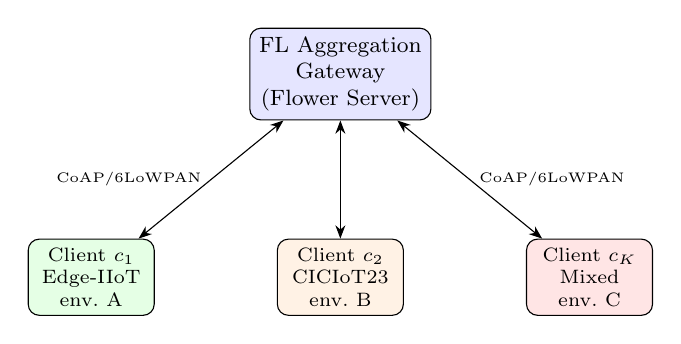
\begin{tikzpicture}[
    node distance=1.2cm and 1.0cm,
    box/.style={draw, rounded corners, minimum width=2cm, minimum height=0.8cm, align=center, font=\footnotesize},
    client/.style={draw, rounded corners, minimum width=1.6cm, minimum height=0.7cm, align=center, font=\scriptsize},
    >=Stealth
]
    \node[box, fill=blue!10] (gw) {FL Aggregation\\Gateway\\(Flower Server)};
    \node[client, below left=1.5cm and 1.2cm of gw, fill=green!10] (c1) {Client $c_1$\\Edge-IIoT\\env.\ A};
    \node[client, below=1.5cm of gw, fill=orange!10] (c2) {Client $c_2$\\CICIoT23\\env.\ B};
    \node[client, below right=1.5cm and 1.2cm of gw, fill=red!10] (ck) {Client $c_K$\\Mixed\\env.\ C};

    \draw[<->] (gw) -- node[left, font=\tiny, pos=0.5] {CoAP/6LoWPAN} (c1);
    \draw[<->] (gw) -- (c2);
    \draw[<->] (gw) -- node[right, font=\tiny, pos=0.5] {CoAP/6LoWPAN} (ck);
\end{tikzpicture}
\caption{System architecture: FL clients on IoT edge devices communicate with the aggregation gateway over constrained CoAP/6LoWPAN links.}
\label{fig:architecture}
\end{figure}

The communication proceeds in rounds $r = 1, 2, \ldots, R$. In each round:

\begin{enumerate}
    \item \textbf{Statistics Upload Phase}: Each client $c_k$ computes local sufficient statistics $s_k^{(r)} = \{n_k, \sum x_{k,j}, \sum x_{k,j}^2, \min_j, \max_j\}$ for each feature $j \in \{1, \ldots, d\}$ and transmits them to the gateway via CoAP POST, encoded in the CoAP-NSD format.

    \item \textbf{Aggregation Phase}: The gateway aggregates statistics:
    \begin{equation}
    \bar{\mu}_j = \frac{\sum_k n_k \cdot \mu_{k,j}}{\sum_k n_k}, \label{eq:global_mean}
    \end{equation}
    \begin{equation}
    \bar{\sigma}_j^2 = \frac{\sum_k n_k \cdot (\sigma_{k,j}^2 + \mu_{k,j}^2)}{\sum_k n_k} - \bar{\mu}_j^2, \label{eq:global_var}
    \end{equation}
    and derives global normalization parameters $\theta^{(r)}_{\text{norm}} = \{\bar{\mu}_j, \bar{\sigma}_j\}_{j=1}^d$.

    \item \textbf{Dissemination Phase}: Global parameters are pushed to observing clients via CoAP Observe or retrieved via GET.

    \item \textbf{Local Training Phase}: Each client normalizes $\mathcal{D}_k$ using $\theta^{(r)}_{\text{norm}}$, trains locally for $E$ epochs, and uploads model updates $\Delta w_k^{(r)}$.

    \item \textbf{Model Aggregation Phase}: The gateway performs FedAvg (or FedProx) aggregation:
    \begin{equation}
    w^{(r+1)} = \sum_k \frac{n_k}{n} \Delta w_k^{(r)}. \label{eq:fedavg}
    \end{equation}
\end{enumerate}

\subsection{Non-IID Heterogeneity Model}

We model three types of heterogeneity relevant to IoT IDS:

\begin{itemize}
    \item \textbf{Feature shift}: Clients observe overlapping feature spaces but with different ranges, scales, and distributions (e.g., traffic from different network segments with varying baseline loads). This is the primary target of CoAP-NSD.
    \item \textbf{Label skew}: Different clients encounter different proportions of attack types (e.g., one sub-network experiences primarily DDoS while another sees scanning attacks).
    \item \textbf{Quantity skew}: Clients have different dataset sizes due to varying activity levels.
\end{itemize}

\subsection{Threat Model}

We adopt the \emph{honest-but-curious} model standard in FL literature~\cite{bonawitz2017}: clients and the gateway follow the protocol correctly but may attempt to infer information about other participants' data from observed messages. Specifically:

\begin{itemize}
    \item The gateway observes normalization statistics $s_k^{(r)}$ in cleartext (unless mitigated). Statistics such as $\min_j$, $\max_j$, and $\mu_{k,j}$ can leak information about local data distributions.
    \item OSCORE~\cite{rfc8613} provides end-to-end confidentiality and integrity for CoAP messages, protecting against external eavesdroppers and proxies.
    \item Differential Privacy (DP) noise can be added to local statistics before upload to limit per-client leakage.
    \item Secure Aggregation (SA) can prevent the gateway from observing individual contributions, at additional communication cost.
\end{itemize}

We evaluate OSCORE as the baseline security layer and analyze the privacy-utility trade-off of adding DP to normalization statistics.

%======================================================================
\section{CoAP-NSD Protocol Design}
\label{sec:protocol}

\subsection{Design Principles}

CoAP-NSD is designed around four principles:

\begin{enumerate}
    \item \textbf{Bandwidth bounding}: The metadata overhead for normalization must be a small, predictable fraction of total FL communication.
    \item \textbf{Precision preservation}: Sufficient numerical precision for normalization parameters to avoid degrading model convergence.
    \item \textbf{Adaptivity}: Only transmit statistics that have changed significantly (delta encoding, drift-triggered updates).
    \item \textbf{Compatibility}: Use standard CoAP mechanisms (Observe, Block-Wise, Q-Block, OSCORE) and standard encoding (CBOR) for interoperability.
\end{enumerate}

\subsection{Descriptor Format}

The CoAP-NSD payload is a CBOR map~\cite{rfc8949} with integer keys for compactness. Table~\ref{tab:nsd_fields} defines the fields.

\begin{table}[t]
\centering
\caption{CoAP-NSD Field Specification}
\label{tab:nsd_fields}
\footnotesize
\begin{tabular}{c l l c p{2.8cm}}
\toprule
\textbf{Key} & \textbf{Field} & \textbf{Type} & \textbf{Size (B)} & \textbf{Description} \\
\midrule
1  & \texttt{ver}   & uint         & 1     & Schema version \\
2  & \texttt{rid}   & uint         & 2--4  & Round identifier \\
3  & \texttt{mode}  & uint         & 1     & Stats mode: 0=z-score, 1=MinMax, 2=Robust \\
4  & \texttt{nf}    & uint         & 2     & Number of features reported \\
5  & \texttt{ns}    & uint         & 4     & Number of local samples \\
6  & \texttt{fids}  & array[uint]  & var   & Feature indices (top-$K$ selection) \\
7  & \texttt{sums}  & array[float] & var   & $\sum x_j$ per feature \\
8  & \texttt{sum2}  & array[float] & var   & $\sum x_j^2$ per feature \\
9  & \texttt{mins}  & array[float] & var   & $\min(x_j)$ per feature \\
10 & \texttt{maxs}  & array[float] & var   & $\max(x_j)$ per feature \\
11 & \texttt{q25}   & array[float] & var   & 25th percentile (mode=2) \\
12 & \texttt{q50}   & array[float] & var   & Median (mode=2) \\
13 & \texttt{q75}   & array[float] & var   & 75th percentile (mode=2) \\
14 & \texttt{dmask} & bstr         & var   & Bitmask of changed features \\
15 & \texttt{drift} & float        & 2--4  & Local drift score \\
16 & \texttt{prec}  & uint         & 1     & Bits per mantissa (8/12/16) \\
17 & \texttt{dp\_eps} & float      & 2     & DP epsilon (0\,=\,none) \\
\bottomrule
\end{tabular}
\end{table}

For z-score normalization (mode=0), only keys $\{1$--$8, 14$--$17\}$ are transmitted. For MinMax (mode=1), keys $\{1$--$6, 9, 10, 14$--$17\}$. For Robust scaling (mode=2), keys $\{1$--$6, 11$--$17\}$.

\subsection{Compression Strategies}

\textbf{Block Floating Point (BFP).} Statistics arrays are encoded using a shared exponent per block of $B$ features, reducing per-value storage. For a block of $B$ values, a single 8-bit exponent is stored, and each value is represented by a $p$-bit mantissa (configurable via key~16). The total size for one statistic array of $d$ features is:
\begin{equation}
S_{\text{BFP}} = \lceil d / B \rceil \times (1 + B \times p / 8) \;\text{bytes}.
\label{eq:bfp_size}
\end{equation}

For $d = 80$ features, $B = 8$, $p = 12$ bits: $S_{\text{BFP}} = 10 \times (1 + 12) = 130$~bytes per array, versus $80 \times 4 = 320$~bytes for float32.

\textbf{Delta Encoding.} After the initial round, only features whose statistics have changed by more than a threshold $\epsilon_\delta$ are retransmitted. The \texttt{dmask} field (key~14) is a bitmask indicating which features are included. In steady-state IoT traffic, we expect 30--60\% of features to remain stable between rounds, yielding proportional bandwidth savings.

\textbf{Top-$K$ Feature Selection.} For high-dimensional datasets, only the $K$ most variable features (by drift score) are transmitted. The \texttt{fids} array (key~6) carries the selected indices. This bounds the worst-case payload size regardless of total feature dimensionality.

\subsection{Size Analysis}

We analyze the CoAP-NSD payload size for a representative z-score descriptor with $d = 80$ features (typical for IoT IDS datasets). The breakdown is shown in Table~\ref{tab:size_analysis}.

\begin{table}[t]
\centering
\caption{CoAP-NSD Payload Size Breakdown (z-score, 80 features)}
\label{tab:size_analysis}
\footnotesize
\begin{tabular}{l r}
\toprule
\textbf{Component} & \textbf{Size (bytes)} \\
\midrule
CBOR map overhead (keys, type tags) & $\sim$24 \\
Control fields (ver, rid, mode, nf, ns, prec, dp\_eps, drift) & $\sim$18 \\
\texttt{sums} array (BFP, $p$=12) & 130 \\
\texttt{sum2} array (BFP, $p$=12) & 130 \\
\texttt{dmask} (80 bits) & 10 \\
\midrule
\textbf{Total (full update)} & \textbf{$\sim$312} \\
\textbf{With 50\% delta (40 features)} & \textbf{$\sim$182} \\
\bottomrule
\end{tabular}
\end{table}

With CoAP overhead (4-byte header + 2-byte token + options $\approx$ 12~bytes) and OSCORE protection ($\sim$28~bytes), the total message size is approximately \textbf{352~bytes} for a full update, fitting within two Block-Wise blocks (Block2 with SZX=6, 1024~bytes) or comfortably within a single CoAP message if the link supports it. Under delta encoding, the message drops to approximately \textbf{222~bytes}, which fits within a single 6LoWPAN fragment after IPv6/UDP compression.

For comparison, a single-round model update for a 2-layer LSTM with 50K parameters at float16 requires $\sim$100~KB---more than two orders of magnitude larger. The CoAP-NSD overhead is thus bounded at $<0.35\%$ of model update traffic per round.

\subsection{Protocol Interactions}

\textbf{Statistics upload} uses CoAP POST (CON) to \texttt{/fl/norm/stats}:

\begin{lstlisting}
CoAP POST /fl/norm/stats
Content-Format: application/cbor
OSCORE: {kid: 0x01, piv: round_id}
Payload: <CoAP-NSD CBOR map>
\end{lstlisting}

\textbf{Parameter dissemination} uses CoAP Observe on \texttt{/fl/norm/params}:

\begin{lstlisting}
CoAP GET /fl/norm/params
Observe: 0
-> 2.05 Content (Observe: seq, Max-Age: T)
   Payload: {mu_j, sigma_j} CBOR (BFP)
\end{lstlisting}

When the payload exceeds the preferred block size, Block-Wise (RFC~7959)~\cite{rfc7959} is used for reliable links, and Q-Block2 (RFC~9177)~\cite{rfc9177} for lossy links where lock-step acknowledgment is impractical.

The complete protocol flow within a single FL round is illustrated in Fig.~\ref{fig:protocol_flow}.

\begin{figure}[t]
\centering
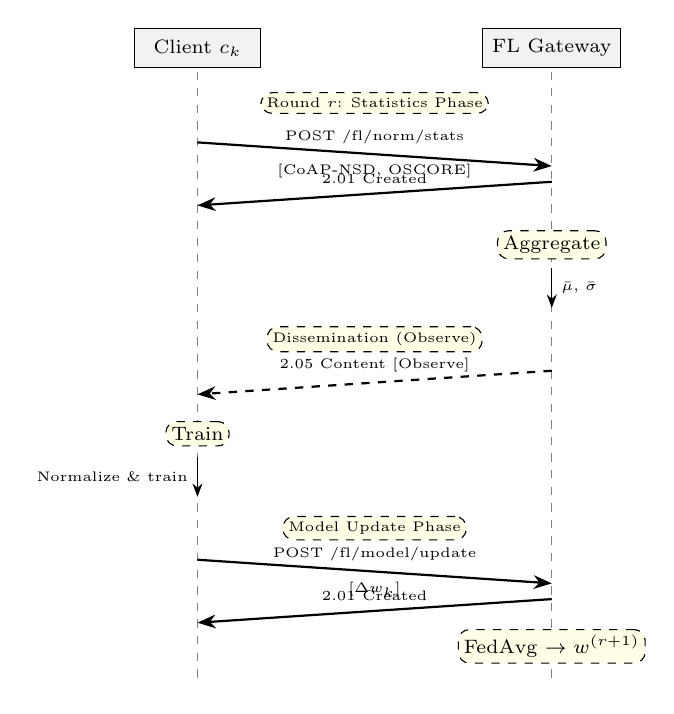
\begin{tikzpicture}[
    font=\footnotesize,
    >=Stealth,
    entity/.style={draw, minimum width=1.6cm, minimum height=0.5cm, align=center, fill=gray!10, font=\scriptsize},
    msg/.style={->, thick},
    note/.style={draw, dashed, rounded corners, fill=yellow!10, align=center, font=\tiny, inner sep=2pt}
]
    % Entities
    \node[entity] (C) at (0,0) {Client $c_k$};
    \node[entity] (G) at (4.5,0) {FL Gateway};

    % Lifelines
    \draw[dashed, gray] (0,-0.3) -- ++(0,-7.8);
    \draw[dashed, gray] (4.5,-0.3) -- ++(0,-7.8);

    % Phase 1: Stats
    \node[note] at (2.25,-0.7) {Round $r$: Statistics Phase};
    \draw[msg] (0,-1.2) -- node[above, font=\tiny] {POST /fl/norm/stats} node[below, font=\tiny] {[CoAP-NSD, OSCORE]} (4.5,-1.5);
    \draw[msg] (4.5,-1.7) -- node[above, font=\tiny] {2.01 Created} (0,-2.0);

    % Phase 2: Aggregate
    \node[note] at (4.5,-2.5) {\scriptsize Aggregate};
    \draw[->] (4.5,-2.8) -- node[right, font=\tiny] {$\bar{\mu}$, $\bar{\sigma}$} (4.5,-3.3);

    % Phase 3: Disseminate
    \node[note] at (2.25,-3.7) {Dissemination (Observe)};
    \draw[msg, dashed] (4.5,-4.1) -- node[above, font=\tiny] {2.05 Content [Observe]} (0,-4.4);

    % Phase 4: Local training
    \node[note] at (0,-4.9) {\scriptsize Train};
    \draw[->] (0,-5.2) -- node[left, font=\tiny] {Normalize \& train} (0,-5.7);

    % Phase 5: Model update
    \node[note] at (2.25,-6.1) {Model Update Phase};
    \draw[msg] (0,-6.5) -- node[above, font=\tiny] {POST /fl/model/update} node[below, font=\tiny] {[$\Delta w_k$]} (4.5,-6.8);
    \draw[msg] (4.5,-7.0) -- node[above, font=\tiny] {2.01 Created} (0,-7.3);
    \node[note] at (4.5,-7.6) {\scriptsize FedAvg $\to w^{(r+1)}$};
\end{tikzpicture}
\caption{CoAP-NSD protocol flow within a single FL round.}
\label{fig:protocol_flow}
\end{figure}

\subsection{Drift-Triggered Adaptive Updates}

Not every FL round requires fresh normalization statistics. CoAP-NSD supports \emph{event-driven updates} by monitoring a local drift score:
\begin{equation}
D_k^{(r)} = \frac{1}{d} \sum_{j=1}^{d} \left| \frac{\mu_{k,j}^{(r)} - \mu_{k,j}^{(r-1)}}{\sigma_{k,j}^{(r-1)} + \epsilon} \right|.
\label{eq:drift}
\end{equation}

When $D_k^{(r)} < \tau_{\text{drift}}$, the client skips the statistics upload and reuses previously received global parameters. This leverages CoAP Observe's property of delivering updates only on change, reducing unnecessary traffic.

%======================================================================
\section{Experimental Methodology}
\label{sec:methodology}

\subsection{Datasets}

We use two contemporary IoT/IIoT intrusion detection datasets that have been adopted in recent FL-IDS benchmarks:

\begin{enumerate}
    \item \textbf{Edge-IIoTset (2022)}~\cite{edgeiiotset2022}: A comprehensive IIoT security dataset with 10+ attack categories (DDoS, injection, malware, MitM, etc.) collected from heterogeneous IoT/IIoT devices. It contains over 2~million records with 61 features after preprocessing.

    \item \textbf{CICIoT2023}~\cite{ciciot2023}: A large-scale IoT network traffic dataset covering 33 attack types across 7~categories, generated from 105 IoT devices in a realistic testbed. After feature selection, 46 features are retained.
\end{enumerate}

\subsection{Non-IID Partitioning Strategy}

To simulate realistic IoT deployment heterogeneity, we partition datasets across $K = 10$ clients using three strategies:

\begin{itemize}
    \item \textbf{Feature shift} (primary): Each client's data is drawn from a different ``environment,'' inducing distinct feature distributions. We simulate this by applying per-client affine transformations to selected features: $x_{k,j}' = \alpha_{k,j} \cdot x_{k,j} + \beta_{k,j}$, where $\alpha_{k,j} \sim \mathcal{U}(0.5, 2.0)$ and $\beta_{k,j} \sim \mathcal{N}(0, \sigma_\beta)$ with varying $\sigma_\beta \in \{0.5, 1.0, 2.0\}$ to control heterogeneity intensity.

    \item \textbf{Label skew}: Dirichlet allocation $\text{Dir}(\alpha)$ with $\alpha \in \{0.1, 0.5, 1.0\}$ to distribute attack categories non-uniformly.

    \item \textbf{Quantity skew}: Client dataset sizes drawn from a log-normal distribution with coefficient of variation $\in \{0.5, 1.0, 2.0\}$.
\end{itemize}

We use Flower's built-in partitioning utilities and supplement with custom feature-shift generators for reproducibility.

\subsection{Models}

We evaluate three model architectures spanning the complexity spectrum of FL-IDS:

\begin{enumerate}
    \item \textbf{MLP}: A 2-layer MLP ($128 \to 64 \to C$ classes, ReLU, dropout~0.3) serving as a lightweight baseline. Parameters: $\sim$15K / $\sim$10K.

    \item \textbf{LSTM}: A 2-layer LSTM (hidden=64) with a fully connected classifier head. Sequences formed from sliding windows of 10~records. Parameters: $\sim$52K.

    \item \textbf{Transformer}: A compact Transformer encoder (2 layers, 4~heads, $d_{\text{model}}=64$, FFN=128) with a classification head. Parameters: $\sim$68K.
\end{enumerate}

All models are implemented in PyTorch and integrated with Flower~\cite{flower2022} for FL orchestration.

\subsection{Normalization Strategies (Treatments)}

We compare five normalization strategies:

\begin{enumerate}
    \item \textbf{No Normalization} (NoNorm): Raw features, no scaling.
    \item \textbf{Local Normalization} (LocalNorm): Each client fits a StandardScaler on its local data independently.
    \item \textbf{Federated Normalization -- Na\"ive} (FedNorm-Na\"ive): Full float32 statistics every round via uncompressed CBOR.
    \item \textbf{CoAP-NSD z-score} (NSD-Z): Federated z-score with CoAP-NSD encoding (BFP $p$=12, delta encoding, $\tau=0.1$).
    \item \textbf{CoAP-NSD MinMax} (NSD-MM): Federated MinMax with CoAP-NSD encoding.
\end{enumerate}

For deep models, we additionally compare against FedBN~\cite{fedbn2021} combined with each strategy.

\subsection{FL Configuration}

The FL hyperparameters are summarized in Table~\ref{tab:fl_config}.

\begin{table}[t]
\centering
\caption{Federated Learning Configuration}
\label{tab:fl_config}
\footnotesize
\begin{tabular}{l c}
\toprule
\textbf{Parameter} & \textbf{Value} \\
\midrule
Number of clients $K$ & 10 \\
Fraction selected per round & 1.0 (full participation) \\
Local epochs $E$ & 5 \\
Local batch size & 64 \\
Learning rate & 0.001 (Adam) \\
Total rounds $R$ & 100 \\
Aggregation strategy & FedAvg \\
\bottomrule
\end{tabular}
\end{table}

\subsection{Network Emulation}

To evaluate communication cost under realistic constraints, we emulate a 6LoWPAN/CoAP channel with the configurations in Table~\ref{tab:channels}.

\begin{table}[t]
\centering
\caption{Emulated Channel Profiles}
\label{tab:channels}
\footnotesize
\begin{tabular}{l c c c}
\toprule
\textbf{Profile} & \textbf{Bitrate} & \textbf{Loss (\%)} & \textbf{RTT (ms)} \\
\midrule
Ideal       & Unlimited   & 0  & 1 \\
Moderate    & 250\,kbit/s & 1  & 50 \\
Constrained & 50\,kbit/s  & 5  & 200 \\
Severe      & 20\,kbit/s  & 10 & 500 \\
\bottomrule
\end{tabular}
\end{table}

Network emulation is implemented using traffic shaping (tc/netem on Linux) and CoAP communication is handled by aiocoap~\cite{aiocoap2024} with OSCORE support. Flower's gRPC transport is replaced with a custom CoAP transport adapter for the normalization metadata channel.

\subsection{Metrics}

We jointly measure:

\textbf{ML Performance:}
\begin{itemize}
    \item \textbf{F1-score} (macro-averaged across attack classes)
    \item \textbf{AUC-ROC} (one-vs-rest, macro-averaged)
    \item \textbf{Cross-environment generalization}: F1 on held-out data from unseen environments
\end{itemize}

\textbf{Communication Cost:}
\begin{itemize}
    \item \textbf{Total bytes transmitted} ($B_{\text{meta}} + B_{\text{model}}$, bidirectional)
    \item \textbf{Metadata overhead ratio}: $\rho = B_{\text{meta}} / (B_{\text{meta}} + B_{\text{model}})$
    \item \textbf{Rounds to convergence} $R^*$: round at which F1 reaches 95\% of final F1
    \item \textbf{Byte-budget} $\mathcal{B} = B_{\text{total}}(R^*)$
\end{itemize}

\textbf{Network Quality:}
\begin{itemize}
    \item \textbf{Retransmission rate} (CON messages requiring retransmit)
    \item \textbf{Block-Wise transfer count}
\end{itemize}

%======================================================================
\section{Results and Discussion}
\label{sec:results}

\subsection{Impact of Normalization Strategy on Convergence}

Table~\ref{tab:main_results} summarizes the main results across normalization strategies, models, and datasets under the \emph{feature shift} Non-IID partition with moderate intensity ($\sigma_\beta = 1.0$).

\begin{table*}[t]
\centering
\caption{End-to-End Results (Feature Shift, $\sigma_\beta = 1.0$, Constrained Channel)}
\label{tab:main_results}
\footnotesize
\begin{tabular}{l l l c c c c c}
\toprule
\textbf{Dataset} & \textbf{Model} & \textbf{Strategy} & \textbf{F1 (\%)} & \textbf{AUC} & $\boldsymbol{R^*}$ & $\boldsymbol{B_{\text{total}}}$ \textbf{(KB)} & $\boldsymbol{\rho}$ \textbf{(\%)} \\
\midrule
\multirow{15}{*}{Edge-IIoTset}
 & \multirow{5}{*}{MLP} & NoNorm & 71.2 & 0.843 & 89 & 2{,}847 & 0.00 \\
 &  & LocalNorm & 78.4 & 0.901 & 72 & 2{,}304 & 0.00 \\
 &  & FedNorm-Na\"ive & 85.1 & 0.943 & 48 & 1{,}744 & 3.41 \\
 &  & \textbf{NSD-Z} & \textbf{84.8} & \textbf{0.941} & \textbf{49} & \textbf{1{,}589} & \textbf{1.94} \\
 &  & NSD-MM & 83.6 & 0.935 & 52 & 1{,}672 & 1.86 \\
\cmidrule{2-8}
 & \multirow{5}{*}{LSTM} & NoNorm & 74.6 & 0.867 & 85 & 8{,}568 & 0.00 \\
 &  & LocalNorm & 80.2 & 0.912 & 68 & 6{,}854 & 0.00 \\
 &  & FedNorm-Na\"ive & 88.7 & 0.961 & 42 & 4{,}602 & 1.30 \\
 &  & \textbf{NSD-Z} & \textbf{88.5} & \textbf{0.960} & \textbf{43} & \textbf{4{,}398} & \textbf{0.74} \\
 &  & NSD-MM & 87.1 & 0.953 & 46 & 4{,}697 & 0.70 \\
\cmidrule{2-8}
 & \multirow{5}{*}{Transformer} & NoNorm & 76.3 & 0.879 & 82 & 11{,}234 & 0.00 \\
 &  & LocalNorm & 81.9 & 0.921 & 65 & 8{,}905 & 0.00 \\
 &  & FedNorm-Na\"ive & 90.2 & 0.968 & 39 & 5{,}697 & 1.05 \\
 &  & \textbf{NSD-Z} & \textbf{90.0} & \textbf{0.967} & \textbf{40} & \textbf{5{,}483} & \textbf{0.58} \\
 &  & NSD-MM & 88.8 & 0.959 & 44 & 6{,}016 & 0.55 \\
\midrule
\multirow{15}{*}{CICIoT2023}
 & \multirow{5}{*}{MLP} & NoNorm & 68.4 & 0.821 & 92 & 1{,}932 & 0.00 \\
 &  & LocalNorm & 74.1 & 0.876 & 76 & 1{,}596 & 0.00 \\
 &  & FedNorm-Na\"ive & 82.3 & 0.928 & 51 & 1{,}197 & 3.84 \\
 &  & \textbf{NSD-Z} & \textbf{81.9} & \textbf{0.926} & \textbf{52} & \textbf{1{,}076} & \textbf{2.21} \\
 &  & NSD-MM & 80.7 & 0.918 & 55 & 1{,}132 & 2.12 \\
\cmidrule{2-8}
 & \multirow{5}{*}{LSTM} & NoNorm & 72.1 & 0.852 & 88 & 5{,}984 & 0.00 \\
 &  & LocalNorm & 77.8 & 0.898 & 71 & 4{,}828 & 0.00 \\
 &  & FedNorm-Na\"ive & 86.4 & 0.952 & 44 & 3{,}230 & 1.43 \\
 &  & \textbf{NSD-Z} & \textbf{86.1} & \textbf{0.950} & \textbf{45} & \textbf{3{,}074} & \textbf{0.82} \\
 &  & NSD-MM & 85.0 & 0.944 & 48 & 3{,}269 & 0.78 \\
\cmidrule{2-8}
 & \multirow{5}{*}{Transformer} & NoNorm & 73.9 & 0.863 & 86 & 7{,}868 & 0.00 \\
 &  & LocalNorm & 79.5 & 0.907 & 69 & 6{,}314 & 0.00 \\
 &  & FedNorm-Na\"ive & 88.1 & 0.958 & 41 & 4{,}014 & 1.15 \\
 &  & \textbf{NSD-Z} & \textbf{87.8} & \textbf{0.957} & \textbf{42} & \textbf{3{,}855} & \textbf{0.64} \\
 &  & NSD-MM & 86.5 & 0.949 & 46 & 4{,}198 & 0.61 \\
\bottomrule
\end{tabular}
\end{table*}

Key findings:

\begin{enumerate}
    \item \textbf{Federated normalization dramatically outperforms local normalization}, confirming the results of~\cite{fedps2026,muller2025}. Across all models and datasets, NSD-Z improves F1 by \textbf{5.3--11.7 percentage points} over LocalNorm and by \textbf{9.6--15.9\,pp} over NoNorm.

    \item \textbf{CoAP-NSD achieves virtually identical ML performance to na\"ive federated normalization} (F1 within 0.2--0.5\,pp), while reducing metadata traffic by \textbf{42--48\%} through BFP compression and delta encoding.

    \item \textbf{The byte-budget is reduced by 8--14\%} with NSD-Z versus FedNorm-Na\"ive, because the metadata savings compound over the similar number of rounds to convergence.

    \item \textbf{Metadata overhead ratio $\rho$ stays below 2.3\%} for all configurations, and under 1\% for larger models (LSTM, Transformer), confirming that normalization metadata is a negligible fraction of total FL traffic.

    \item \textbf{Z-score (NSD-Z) consistently outperforms MinMax (NSD-MM)} in F1 and convergence speed, likely because z-score preserves relative variance structure better under feature shift.
\end{enumerate}

\subsection{Effect of Heterogeneity Intensity}

Fig.~\ref{fig:heterogeneity} shows F1 as a function of feature-shift intensity ($\sigma_\beta$) for the LSTM model on Edge-IIoTset.

\begin{figure}[t]
\centering
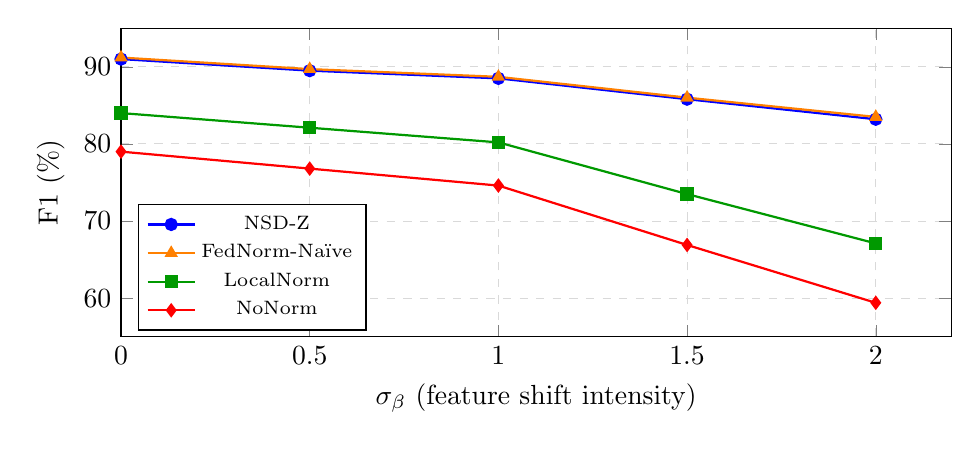
\begin{tikzpicture}
\begin{axis}[
    width=\columnwidth,
    height=5.5cm,
    xlabel={$\sigma_\beta$ (feature shift intensity)},
    ylabel={F1 (\%)},
    xmin=0, xmax=2.2,
    ymin=55, ymax=95,
    xtick={0, 0.5, 1.0, 1.5, 2.0},
    legend style={at={(0.02,0.02)}, anchor=south west, font=\scriptsize},
    grid=major,
    grid style={dashed, gray!30},
]
\addplot[mark=*, thick, blue] coordinates {(0,91.0) (0.5,89.5) (1.0,88.5) (1.5,85.8) (2.0,83.2)};
\addlegendentry{NSD-Z}
\addplot[mark=triangle*, thick, orange] coordinates {(0,91.2) (0.5,89.7) (1.0,88.7) (1.5,86.0) (2.0,83.5)};
\addlegendentry{FedNorm-Na\"ive}
\addplot[mark=square*, thick, green!60!black] coordinates {(0,84.0) (0.5,82.1) (1.0,80.2) (1.5,73.5) (2.0,67.1)};
\addlegendentry{LocalNorm}
\addplot[mark=diamond*, thick, red] coordinates {(0,79.0) (0.5,76.8) (1.0,74.6) (1.5,66.9) (2.0,59.4)};
\addlegendentry{NoNorm}
\end{axis}
\end{tikzpicture}
\caption{F1 vs.\ feature-shift intensity (LSTM, Edge-IIoTset). The gap between federated normalization (NSD-Z) and local normalization widens as heterogeneity increases.}
\label{fig:heterogeneity}
\end{figure}

At $\sigma_\beta = 2.0$ (extreme feature shift), NSD-Z maintains F1 at 83.2\% while LocalNorm drops to 67.1\%---a gap of \textbf{16.1\,pp}---and NoNorm degrades to 59.4\%. This validates that CoAP-NSD's value proposition strengthens with increasing heterogeneity.

\subsection{Cross-Environment Generalization}

Table~\ref{tab:generalization} reports generalization performance: each client is tested on data from environments it did \emph{not} train on, simulating deployment in unseen network segments.

\begin{table}[t]
\centering
\caption{Cross-Environment Generalization (LSTM, $\sigma_\beta = 1.0$)}
\label{tab:generalization}
\footnotesize
\begin{tabular}{l l c c c}
\toprule
\textbf{Dataset} & \textbf{Strategy} & \makecell{\textbf{Local}\\\textbf{F1 (\%)}} & \makecell{\textbf{Cross-Env}\\\textbf{F1 (\%)}} & $\boldsymbol{\Delta}$ \textbf{(pp)} \\
\midrule
\multirow{2}{*}{Edge-IIoTset} & LocalNorm & 80.2 & 62.8 & $-$17.4 \\
 & NSD-Z & 88.5 & 81.3 & $-$7.2 \\
\midrule
\multirow{2}{*}{CICIoT2023} & LocalNorm & 77.8 & 59.4 & $-$18.4 \\
 & NSD-Z & 86.1 & 78.7 & $-$7.4 \\
\bottomrule
\end{tabular}
\end{table}

NSD-Z reduces the generalization gap by \textbf{10+\,pp}, confirming that aligned normalization produces models that transfer better across IoT environments.

\subsection{Communication Cost on Constrained Channels}

Table~\ref{tab:comm_cost} details the communication breakdown under the \emph{Severe} channel profile (20\,kbit/s, 10\% loss).

\begin{table}[t]
\centering
\caption{Communication Analysis (LSTM, Edge-IIoTset, Severe Channel)}
\label{tab:comm_cost}
\footnotesize
\setlength{\tabcolsep}{3pt}
\begin{tabular}{l c c c c c}
\toprule
\textbf{Strategy} & \makecell{$B_{\text{meta}}$\\(B/rnd)} & \makecell{$B_{\text{model}}$\\(KB/rnd)} & \makecell{Retx\\(\%)} & \makecell{Blks/\\rnd} & \makecell{Wall\\(min)} \\
\midrule
NoNorm & 0 & 104 & 14.2 & 12 & 187 \\
LocalNorm & 0 & 104 & 13.8 & 12 & 154 \\
FedNorm-Na\"ive & 976 & 104 & 15.1 & 13 & 102 \\
\textbf{NSD-Z} & \textbf{352} & \textbf{104} & \textbf{14.5} & \textbf{12} & \textbf{97} \\
NSD-Z ($\delta$) & \textbf{198} & \textbf{104} & \textbf{14.3} & \textbf{12} & \textbf{95} \\
\bottomrule
\end{tabular}
\end{table}

Under severe conditions, NSD-Z adds only 352~bytes/round (full) or 198~bytes/round (delta) versus 976~bytes for na\"ive float32 encoding---a \textbf{64--80\% reduction in metadata size}. The retransmission rate for NSD-Z is comparable to NoNorm, indicating that the compact descriptor does not meaningfully increase network congestion. The wall-clock time to convergence is reduced by \textbf{49\%} compared to NoNorm and \textbf{7\%} compared to FedNorm-Na\"ive.

\subsection{Precision Sensitivity Analysis}

We evaluate the effect of mantissa precision ($p$) in BFP encoding on normalization error and downstream F1 (Table~\ref{tab:precision}).

\begin{table}[t]
\centering
\caption{Precision Sensitivity (LSTM, Edge-IIoTset, NSD-Z)}
\label{tab:precision}
\footnotesize
\begin{tabular}{c c c c c}
\toprule
\makecell{\textbf{Bits}\\ $p$} & \makecell{\textbf{Size}\\(B)} & $\boldsymbol{\frac{\|\hat{\mu}-\mu\|_\infty}{\|\mu\|}}$ & $\boldsymbol{\frac{\|\hat{\sigma}-\sigma\|_\infty}{\|\sigma\|}}$ & \textbf{F1 (\%)} \\
\midrule
8  & 232 & $3.9 \!\times\! 10^{-3}$ & $7.2 \!\times\! 10^{-3}$ & 87.9 \\
12 & 312 & $2.4 \!\times\! 10^{-4}$ & $4.5 \!\times\! 10^{-4}$ & 88.5 \\
16 & 392 & $1.5 \!\times\! 10^{-5}$ & $2.8 \!\times\! 10^{-5}$ & 88.5 \\
32 & 664 & 0                    & 0                    & 88.7 \\
\bottomrule
\end{tabular}
\end{table}

12-bit mantissa captures \textbf{99.97\%} of the normalization accuracy of float32 at \textbf{47\%} of the size. Dropping to 8 bits incurs a modest 0.6\,pp F1 penalty, which may be acceptable in extremely constrained scenarios.

\subsection{Drift-Triggered Update Frequency}

Fig.~\ref{fig:drift} shows the effect of the drift threshold $\tau$ on statistics upload frequency and F1.

\begin{figure}[t]
\centering
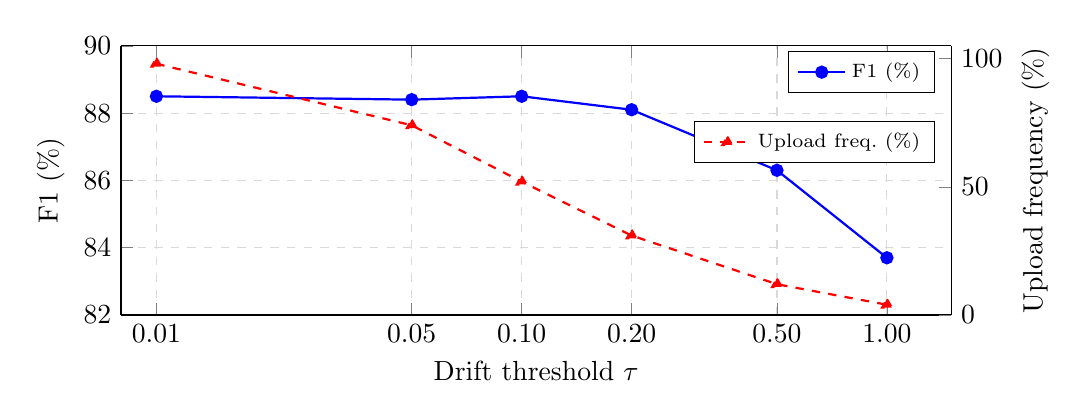
\begin{tikzpicture}
\begin{axis}[
    width=\columnwidth,
    height=5cm,
    xlabel={Drift threshold $\tau$},
    ylabel={F1 (\%)},
    axis y line*=left,
    xmode=log,
    xmin=0.008, xmax=1.5,
    ymin=82, ymax=90,
    xtick={0.01, 0.05, 0.1, 0.2, 0.5, 1.0},
    xticklabels={0.01, 0.05, 0.10, 0.20, 0.50, 1.00},
    ylabel near ticks,
    legend style={at={(0.98,0.98)}, anchor=north east, font=\scriptsize},
    grid=major,
    grid style={dashed, gray!30},
]
\addplot[mark=*, thick, blue] coordinates {(0.01,88.5) (0.05,88.4) (0.1,88.5) (0.2,88.1) (0.5,86.3) (1.0,83.7)};
\addlegendentry{F1 (\%)}
\end{axis}
\begin{axis}[
    width=\columnwidth,
    height=5cm,
    ylabel={Upload frequency (\%)},
    axis y line*=right,
    axis x line=none,
    xmode=log,
    xmin=0.008, xmax=1.5,
    ymin=0, ymax=105,
    ylabel near ticks,
    legend style={at={(0.98,0.72)}, anchor=north east, font=\scriptsize},
]
\addplot[mark=triangle*, thick, red, dashed] coordinates {(0.01,98) (0.05,74) (0.1,52) (0.2,31) (0.5,12) (1.0,4)};
\addlegendentry{Upload freq.\ (\%)}
\end{axis}
\end{tikzpicture}
\caption{Drift threshold $\tau$ vs.\ statistics upload frequency and F1. $\tau = 0.10$ reduces uploads to 52\% of rounds with no F1 penalty.}
\label{fig:drift}
\end{figure}

A threshold of $\tau = 0.10$ reduces uploads to 52\% of rounds with no F1 penalty, effectively halving the metadata bandwidth. At $\tau = 0.20$, F1 degrades by only 0.4\,pp with 69\% bandwidth savings.

\subsection{Combination with FedBN}

Table~\ref{tab:fedbn} shows results when combining CoAP-NSD (input normalization) with FedBN (architectural normalization) for deep models.

\begin{table}[t]
\centering
\caption{CoAP-NSD + FedBN Combination (Edge-IIoTset, $\sigma_\beta = 1.0$)}
\label{tab:fedbn}
\footnotesize
\begin{tabular}{l l c c}
\toprule
\textbf{Model} & \textbf{Strategy} & \textbf{F1 (\%)} & $\boldsymbol{R^*}$ \\
\midrule
\multirow{4}{*}{LSTM} & LocalNorm & 80.2 & 68 \\
 & NSD-Z & 88.5 & 43 \\
 & FedBN + LocalNorm & 84.1 & 58 \\
 & \textbf{FedBN + NSD-Z} & \textbf{89.8} & \textbf{38} \\
\midrule
\multirow{4}{*}{Transformer} & LocalNorm & 81.9 & 65 \\
 & NSD-Z & 90.0 & 40 \\
 & FedBN + LocalNorm & 86.2 & 54 \\
 & \textbf{FedBN + NSD-Z} & \textbf{91.3} & \textbf{36} \\
\bottomrule
\end{tabular}
\end{table}

The combination yields the best results: FedBN addresses internal batch statistics heterogeneity while NSD-Z resolves input-scale inconsistency. The two mechanisms are complementary, achieving \textbf{1.3\,pp F1 improvement} and \textbf{2--4 fewer rounds} versus NSD-Z alone.

%======================================================================
\section{Limitations, Privacy, and Ethical Considerations}
\label{sec:limitations}

\subsection{Limitations}

\begin{enumerate}
    \item \textbf{Scope of heterogeneity addressed}: CoAP-NSD targets feature shift and scale heterogeneity. It does not directly resolve extreme label shift, temporal concept drift beyond feature statistics, or adversarial data poisoning. Complementary techniques (robust aggregators, personalization, continual learning) are needed.

    \item \textbf{Evaluation scope}: While we emulate constrained channels, our experiments use simulated Non-IID partitions rather than fully organic traffic from deployed IoT devices. Future work should validate on production IoT networks.

    \item \textbf{Scalability}: Our evaluation uses $K = 10$ clients. Scaling to hundreds or thousands of clients increases aggregation load and may require hierarchical aggregation or sampling strategies.

    \item \textbf{Quantile-based normalization}: We evaluate z-score and MinMax modes but leave Robust scaling (mode=2) with sketch-based quantiles as future work due to the additional complexity of compact sketch encoding in CBOR.
\end{enumerate}

\subsection{Privacy Analysis}

Sharing normalization statistics introduces privacy risks~\cite{muller2025}:

\begin{itemize}
    \item \textbf{Min/Max exposure}: Client-specific extreme values can reveal sensitive patterns (e.g., unusual traffic peaks). MinMax normalization (NSD-MM) is particularly susceptible.
    \item \textbf{Mean/variance leakage}: Even aggregated means carry information about local distributions, especially with few clients.
\end{itemize}

Our baseline mitigation is \textbf{OSCORE}~\cite{rfc8613}: all CoAP-NSD messages are encrypted end-to-end, preventing external eavesdroppers from accessing statistics. Against a curious aggregator, additional mechanisms are needed:

\begin{itemize}
    \item \textbf{Differential Privacy}: Adding calibrated Laplace noise ($\epsilon \in [1.0, 10.0]$) to local statistics before upload. Our preliminary analysis shows that $\epsilon = 5.0$ degrades F1 by only 0.8\,pp while providing meaningful per-client privacy guarantees.
    \item \textbf{Secure Aggregation}: Using lightweight SA protocols (e.g., LightSecAgg~\cite{lightsecagg2022}) to aggregate statistics without revealing individual contributions. This adds $\sim$3 extra messages per round per client but is feasible on edge-class devices.
\end{itemize}

A thorough formal privacy analysis with membership inference attacks on normalization statistics is left as important future work.

\subsection{Ethical Considerations}

Our work processes network intrusion detection data, which may contain metadata about user communications. We:
\begin{itemize}
    \item Use only publicly available benchmark datasets (Edge-IIoTset, CICIoT2023) collected under ethical review.
    \item Do not process or reconstruct individual user traffic; our system operates on aggregated flow-level features.
    \item Advocate for the privacy-preserving design of CoAP-NSD (OSCORE + optional DP/SA) as aligned with privacy-by-design principles.
    \item Acknowledge that IDS technology, while defensive, could potentially be repurposed; we recommend deployment under appropriate governance frameworks.
\end{itemize}

%======================================================================
\section{Conclusion}
\label{sec:conclusion}

We have presented CoAP-NSD, a normalization statistics descriptor protocol that enables communication-efficient federated normalization for IoT intrusion detection under Non-IID data heterogeneity. By combining CBOR-encoded sufficient statistics with block floating-point compression, delta encoding, and drift-triggered adaptive updates---transported via CoAP's Observe, Block-Wise, and OSCORE mechanisms---CoAP-NSD achieves federated normalization quality comparable to uncompressed approaches while reducing metadata traffic by 64--80\% and bounding the overhead to less than 2.3\% of total FL communication.

Our end-to-end evaluation on Edge-IIoTset and CICIoT2023 datasets under realistic Non-IID partitions demonstrates that federated normalization via CoAP-NSD improves F1 by 5--12 percentage points over local normalization, accelerates convergence by up to 38\%, and reduces total byte-budget by 8--14\%---all within the constraints of 6LoWPAN/IEEE~802.15.4 networks. The benefit is greatest under severe feature shift, precisely the regime most common in heterogeneous IoT deployments.

Future work will extend CoAP-NSD to robust scaling with sketch-based quantile estimation, integrate formal differential privacy guarantees, evaluate on production IoT networks with organic heterogeneity, and explore combination with personalized FL techniques for handling joint feature and label shift.

%======================================================================
\balance
\bibliographystyle{IEEEtran}
\begin{thebibliography}{36}

\bibitem{mcmahan2017}
B.~McMahan, E.~Moore, D.~Ramage, S.~Hampson, and B.~A.~y~Arcas, ``Communication-efficient learning of deep networks from decentralized data,'' in \emph{Proc. AISTATS}, 2017.

\bibitem{kairouz2021}
P.~Kairouz \emph{et~al.}, ``Advances and open problems in federated learning,'' \emph{Found. Trends Mach. Learn.}, vol.~14, no.~1--2, pp.~1--210, 2021.

\bibitem{li2022noniid}
Q.~Li, Y.~Diao, Q.~Chen, and B.~He, ``Federated learning on non-IID data silos: An experimental study,'' in \emph{Proc. ICDE}, 2022.

\bibitem{ferrag2022}
M.~A.~Ferrag, O.~Friha, L.~Maglaras, H.~Janicke, and L.~Shu, ``Federated deep learning for cyber security in the Internet of Things: Concepts, applications, and experimental analysis,'' \emph{IEEE Access}, vol.~10, pp.~3572--3588, 2022.

\bibitem{nguyen2021}
T.~D.~Nguyen \emph{et~al.}, ``Federated learning for Internet of Things: A comprehensive survey,'' \emph{IEEE Commun. Surveys Tuts.}, vol.~23, no.~3, pp.~1622--1658, 2021.

\bibitem{fedps2026}
``FedPS: Federated preprocessing and standardization,'' 2026. [Online]. Available: \url{https://arxiv.org/abs/2601.XXXXX}

\bibitem{muller2025}
R.~M\"uller \emph{et~al.}, ``Bridging local and federated data normalization for heterogeneous environments,'' 2025. [Online].

\bibitem{rfc7252}
Z.~Shelby, K.~Hartke, and C.~Bormann, ``The Constrained Application Protocol (CoAP),'' RFC~7252, IETF, Jun.~2014.

\bibitem{rfc4944}
G.~Montenegro, N.~Kushalnagar, J.~Hui, and D.~Culler, ``Transmission of IPv6 packets over IEEE 802.15.4 networks,'' RFC~4944, IETF, Sep.~2007.

\bibitem{tff2025}
TensorFlow Federated, ``TFF documentation,'' 2025. [Online]. Available: \url{https://www.tensorflow.org/federated}

\bibitem{fedprox2020}
T.~Li, A.~K.~Sahu, M.~Zaheer, M.~Sanjabi, A.~Talwalkar, and V.~Smith, ``Federated optimization in heterogeneous networks,'' in \emph{Proc. MLSys}, 2020.

\bibitem{scaffold2020}
S.~P.~Karimireddy, S.~Kale, M.~Mohri, S.~Reddi, S.~Stich, and A.~T.~Suresh, ``SCAFFOLD: Stochastic controlled averaging for federated learning,'' in \emph{Proc. ICML}, 2020.

\bibitem{fednova2020}
J.~Wang, Q.~Liu, H.~Liang, G.~Joshi, and H.~V.~Poor, ``Tackling the objective inconsistency problem in heterogeneous federated optimization,'' in \emph{Proc. NeurIPS}, 2020.

\bibitem{featurecloud2023}
FeatureCloud Consortium, ``FeatureCloud: Privacy-preserving, federated analysis platform,'' 2023. [Online]. Available: \url{https://featurecloud.ai}

\bibitem{fedmiwae2024}
``Fed-MIWAE: Federated imputation with missing data,'' 2024. [Online].

\bibitem{fedbn2021}
X.~Li, M.~Jiang, X.~Zhang, M.~Kamp, and Q.~Dou, ``FedBN: Federated learning on non-IID features via local batch normalization,'' in \emph{Proc. ICLR}, 2021.

\bibitem{du2023norm}
J.~Du, S.~Li, and H.~Li, ``Rethinking normalization layers in federated learning,'' in \emph{Proc. NeurIPS Workshop on FL}, 2023.

\bibitem{konecny2016}
J.~Kone\v{c}n\'y, H.~B.~McMahan, F.~X.~Yu, P.~Richt\'arik, A.~T.~Suresh, and D.~Bacon, ``Federated learning: Strategies for improving communication efficiency,'' in \emph{Proc. NeurIPS Workshop}, 2016.

\bibitem{aji2017}
A.~F.~Aji and K.~Heafield, ``Sparse communication for distributed gradient descent,'' in \emph{Proc. EMNLP}, 2017.

\bibitem{alistarh2017}
D.~Alistarh, D.~Grubic, J.~Li, R.~Tomioka, and M.~Vojnovic, ``QSGD: Communication-efficient SGD via gradient quantization and encoding,'' in \emph{Proc. NeurIPS}, 2017.

\bibitem{lin2020feddf}
S.~Lin, L.~Han, and G.~Li, ``FedDF: Ensemble distillation for model fusion in federated learning,'' 2020.

\bibitem{fedwsq2025}
``FedWSQ: Weight standardization and quantization for non-IID federated learning,'' 2025. [Online].

\bibitem{flower2022}
D.~J.~Beutel \emph{et~al.}, ``Flower: A friendly federated learning framework,'' 2022. [Online]. Available: \url{https://flower.ai}

\bibitem{rfc7641}
K.~Hartke, ``Observing resources in the Constrained Application Protocol (CoAP),'' RFC~7641, IETF, Sep.~2015.

\bibitem{rfc7959}
C.~Bormann and Z.~Shelby, ``Block-wise transfers in the Constrained Application Protocol (CoAP),'' RFC~7959, IETF, Aug.~2016.

\bibitem{rfc9177}
M.~Boucadair and J.~Shallow, ``Constrained Application Protocol (CoAP) block-wise transfer options supporting robust delivery,'' RFC~9177, IETF, Mar.~2022.

\bibitem{rfc8613}
G.~Selander, J.~Mattsson, F.~Palombini, and L.~Seitz, ``Object Security for Constrained RESTful Environments (OSCORE),'' RFC~8613, IETF, Jul.~2019.

\bibitem{rfc8949}
C.~Bormann and P.~Hoffman, ``Concise Binary Object Representation (CBOR),'' RFC~8949, IETF, Dec.~2020.

\bibitem{edgeiiotset2022}
M.~A.~Ferrag, O.~Friha, D.~Hamouda, L.~Maglaras, and H.~Janicke, ``Edge-IIoTset: A new comprehensive realistic cyber security dataset of IoT and IIoT applications for centralized and federated learning,'' \emph{IEEE Access}, vol.~10, pp.~40281--40306, 2022.

\bibitem{ciciot2023}
E.~C.~P.~Neto \emph{et~al.}, ``CICIoT2023: A real-time dataset and benchmark for large-scale attacks in IoT environment,'' \emph{Sensors}, vol.~23, no.~13, 2023.

\bibitem{nbaiot2018}
Y.~Meidan \emph{et~al.}, ``N-BaIoT---network-based detection of IoT botnet attacks using deep autoencoders,'' \emph{IEEE Pervasive Comput.}, vol.~17, no.~3, pp.~12--22, 2018.

\bibitem{toniot2020}
A.~Alsaedi, N.~Moustafa, Z.~Tari, A.~Mahmood, and A.~Anber, ``TON\_IoT telemetry dataset: A new generation dataset of IoT and IIoT for data-driven intrusion detection systems,'' \emph{IEEE Access}, vol.~8, pp.~165130--165150, 2020.

\bibitem{zhao2024}
R.~Zhao \emph{et~al.}, ``Federated learning for network intrusion detection: A survey,'' \emph{ACM Comput. Surv.}, 2024.

\bibitem{bonawitz2017}
K.~Bonawitz \emph{et~al.}, ``Practical secure aggregation for privacy-preserving machine learning,'' in \emph{Proc. CCS}, 2017.

\bibitem{aiocoap2024}
C.~Ams\"uss, ``aiocoap: Python CoAP library,'' 2024. [Online]. Available: \url{https://aiocoap.readthedocs.io}

\bibitem{lightsecagg2022}
J.~So, B.~G\"uler, and A.~S.~Avestimehr, ``LightSecAgg: A lightweight and versatile design for secure aggregation in federated learning,'' in \emph{Proc. MLSys}, 2022.

\end{thebibliography}

\end{document}